\documentclass{book}
\usepackage[a4paper,top=2.5cm,bottom=2.5cm,left=2.5cm,right=2.5cm]{geometry}
\usepackage{makeidx}
\usepackage{natbib}
\usepackage{graphicx}
\usepackage{multicol}
\usepackage{float}
\usepackage{listings}
\usepackage{color}
\usepackage{ifthen}
\usepackage[table]{xcolor}
\usepackage{textcomp}
\usepackage{alltt}
\usepackage{ifpdf}
\ifpdf
\usepackage[pdftex,
            pagebackref=true,
            colorlinks=true,
            linkcolor=blue,
            unicode
           ]{hyperref}
\else
\usepackage[ps2pdf,
            pagebackref=true,
            colorlinks=true,
            linkcolor=blue,
            unicode
           ]{hyperref}
\usepackage{pspicture}
\fi
\usepackage[utf8]{inputenc}
\usepackage{mathptmx}
\usepackage[scaled=.90]{helvet}
\usepackage{courier}
\usepackage{sectsty}
\usepackage{amssymb}
\usepackage[titles]{tocloft}
\usepackage{doxygen}
\lstset{language=C++,inputencoding=utf8,basicstyle=\footnotesize,breaklines=true,breakatwhitespace=true,tabsize=4,numbers=left }
\makeindex
\setcounter{tocdepth}{3}
\renewcommand{\footrulewidth}{0.4pt}
\renewcommand{\familydefault}{\sfdefault}
\hfuzz=15pt
\setlength{\emergencystretch}{15pt}
\hbadness=750
\tolerance=750
\begin{document}
\hypersetup{pageanchor=false,citecolor=blue}
\begin{titlepage}
\vspace*{7cm}
\begin{center}
{\Large C\-M2301 }\\
\vspace*{1cm}
{\large Generated by Doxygen 1.8.3}\\
\vspace*{0.5cm}
{\small Tue Jan 8 2013 01:38:13}\\
\end{center}
\end{titlepage}
\clearemptydoublepage
\pagenumbering{roman}
\tableofcontents
\clearemptydoublepage
\pagenumbering{arabic}
\hypersetup{pageanchor=true,citecolor=blue}
\chapter{Hierarchical Index}
\section{Class Hierarchy}
This inheritance list is sorted roughly, but not completely, alphabetically\-:\begin{DoxyCompactList}
\item list\begin{DoxyCompactList}
\item \contentsline{section}{queue.\-Queue\-Manager}{\pageref{classqueue_1_1_queue_manager}}{}
\end{DoxyCompactList}
\item \contentsline{section}{Learn.\-old\-\_\-models.\-admin.\-Admin.\-Meta}{\pageref{class_learn_1_1old__models_1_1admin_1_1_admin_1_1_meta}}{}
\item \contentsline{section}{Learn.\-old\-\_\-models.\-lecture.\-Lecture.\-Meta}{\pageref{class_learn_1_1old__models_1_1lecture_1_1_lecture_1_1_meta}}{}
\item \contentsline{section}{Learn.\-old\-\_\-models.\-lecturer.\-Lecturer.\-Meta}{\pageref{class_learn_1_1old__models_1_1lecturer_1_1_lecturer_1_1_meta}}{}
\item \contentsline{section}{Learn.\-old\-\_\-models.\-queue.\-Queue.\-Meta}{\pageref{class_learn_1_1old__models_1_1queue_1_1_queue_1_1_meta}}{}
\item \contentsline{section}{Learn.\-old\-\_\-models.\-student.\-Student.\-Meta}{\pageref{class_learn_1_1old__models_1_1student_1_1_student_1_1_meta}}{}
\item \contentsline{section}{Learn.\-old\-\_\-models.\-user.\-User.\-Meta}{\pageref{class_learn_1_1old__models_1_1user_1_1_user_1_1_meta}}{}
\item Model\begin{DoxyCompactList}
\item \contentsline{section}{Learn.\-models.\-Base}{\pageref{class_learn_1_1models_1_1_base}}{}
\begin{DoxyCompactList}
\item \contentsline{section}{Learn.\-models.\-Answer}{\pageref{class_learn_1_1models_1_1_answer}}{}
\item \contentsline{section}{Learn.\-models.\-Attachment}{\pageref{class_learn_1_1models_1_1_attachment}}{}
\item \contentsline{section}{Learn.\-models.\-Config}{\pageref{class_learn_1_1models_1_1_config}}{}
\item \contentsline{section}{Learn.\-models.\-Course}{\pageref{class_learn_1_1models_1_1_course}}{}
\item \contentsline{section}{Learn.\-models.\-Event\-Log}{\pageref{class_learn_1_1models_1_1_event_log}}{}
\item \contentsline{section}{Learn.\-models.\-Lecture}{\pageref{class_learn_1_1models_1_1_lecture}}{}
\item \contentsline{section}{Learn.\-models.\-Link}{\pageref{class_learn_1_1models_1_1_link}}{}
\item \contentsline{section}{Learn.\-models.\-Module}{\pageref{class_learn_1_1models_1_1_module}}{}
\item \contentsline{section}{Learn.\-models.\-Question}{\pageref{class_learn_1_1models_1_1_question}}{}
\item \contentsline{section}{Learn.\-models.\-Result}{\pageref{class_learn_1_1models_1_1_result}}{}
\item \contentsline{section}{Learn.\-models.\-Revision}{\pageref{class_learn_1_1models_1_1_revision}}{}
\item \contentsline{section}{Learn.\-models.\-Test}{\pageref{class_learn_1_1models_1_1_test}}{}
\item \contentsline{section}{Learn.\-models.\-Test\-Instance}{\pageref{class_learn_1_1models_1_1_test_instance}}{}
\item \contentsline{section}{Learn.\-models.\-User}{\pageref{class_learn_1_1models_1_1_user}}{}
\item \contentsline{section}{Learn.\-models.\-User\-Field}{\pageref{class_learn_1_1models_1_1_user_field}}{}
\item \contentsline{section}{Learn.\-models.\-Video}{\pageref{class_learn_1_1models_1_1_video}}{}
\item \contentsline{section}{Learn.\-models.\-Video\-Format}{\pageref{class_learn_1_1models_1_1_video_format}}{}
\end{DoxyCompactList}
\item \contentsline{section}{Learn.\-old\-\_\-models.\-lecture.\-Lecture}{\pageref{class_learn_1_1old__models_1_1lecture_1_1_lecture}}{}
\item \contentsline{section}{Learn.\-old\-\_\-models.\-queue.\-Queue}{\pageref{class_learn_1_1old__models_1_1queue_1_1_queue}}{}
\item \contentsline{section}{Learn.\-old\-\_\-models.\-user.\-User}{\pageref{class_learn_1_1old__models_1_1user_1_1_user}}{}
\end{DoxyCompactList}
\item object\begin{DoxyCompactList}
\item \contentsline{section}{queue.\-Database}{\pageref{classqueue_1_1_database}}{}
\item \contentsline{section}{queue.\-Queue\-Item}{\pageref{classqueue_1_1_queue_item}}{}
\item \contentsline{section}{server\-\_\-load.\-Server\-Load}{\pageref{classserver__load_1_1_server_load}}{}
\end{DoxyCompactList}
\item Test\-Case\begin{DoxyCompactList}
\item \contentsline{section}{Learn.\-tests.\-Simple\-Test}{\pageref{class_learn_1_1tests_1_1_simple_test}}{}
\end{DoxyCompactList}
\item User\begin{DoxyCompactList}
\item \contentsline{section}{Learn.\-old\-\_\-models.\-admin.\-Admin}{\pageref{class_learn_1_1old__models_1_1admin_1_1_admin}}{}
\item \contentsline{section}{Learn.\-old\-\_\-models.\-lecturer.\-Lecturer}{\pageref{class_learn_1_1old__models_1_1lecturer_1_1_lecturer}}{}
\item \contentsline{section}{Learn.\-old\-\_\-models.\-student.\-Student}{\pageref{class_learn_1_1old__models_1_1student_1_1_student}}{}
\end{DoxyCompactList}
\end{DoxyCompactList}

\chapter{Class Index}
\section{Class List}
Here are the classes, structs, unions and interfaces with brief descriptions\-:\begin{DoxyCompactList}
\item\contentsline{section}{\hyperlink{class_learn_1_1old__models_1_1admin_1_1_admin}{Learn.\-old\-\_\-models.\-admin.\-Admin} }{\pageref{class_learn_1_1old__models_1_1admin_1_1_admin}}{}
\item\contentsline{section}{\hyperlink{class_learn_1_1models_1_1_answer}{Learn.\-models.\-Answer} \\*An instance of the \hyperlink{class_learn_1_1models_1_1_answer}{Answer} class will hold text associated with an answer, and whether or not the answer is correct or not }{\pageref{class_learn_1_1models_1_1_answer}}{}
\item\contentsline{section}{\hyperlink{class_learn_1_1models_1_1_attachment}{Learn.\-models.\-Attachment} \\*An \hyperlink{class_learn_1_1models_1_1_attachment}{Attachment} is a collection of revisions }{\pageref{class_learn_1_1models_1_1_attachment}}{}
\item\contentsline{section}{\hyperlink{class_learn_1_1models_1_1_base}{Learn.\-models.\-Base} \\*\hyperlink{class_learn_1_1models_1_1_base}{Base} class containing common properties and methods for models }{\pageref{class_learn_1_1models_1_1_base}}{}
\item\contentsline{section}{\hyperlink{class_learn_1_1models_1_1_config}{Learn.\-models.\-Config} \\*Contains configuration and preferences for the system }{\pageref{class_learn_1_1models_1_1_config}}{}
\item\contentsline{section}{\hyperlink{class_learn_1_1models_1_1_course}{Learn.\-models.\-Course} \\*A course represents a top level definition of a degree, they are a collection of modules }{\pageref{class_learn_1_1models_1_1_course}}{}
\item\contentsline{section}{\hyperlink{classqueue_1_1_database}{queue.\-Database} }{\pageref{classqueue_1_1_database}}{}
\item\contentsline{section}{\hyperlink{class_learn_1_1models_1_1_event_log}{Learn.\-models.\-Event\-Log} \\*Handles the storing of events in the log }{\pageref{class_learn_1_1models_1_1_event_log}}{}
\item\contentsline{section}{\hyperlink{class_learn_1_1models_1_1_lecture}{Learn.\-models.\-Lecture} \\*Represents a lecture within a module }{\pageref{class_learn_1_1models_1_1_lecture}}{}
\item\contentsline{section}{\hyperlink{class_learn_1_1old__models_1_1lecture_1_1_lecture}{Learn.\-old\-\_\-models.\-lecture.\-Lecture} }{\pageref{class_learn_1_1old__models_1_1lecture_1_1_lecture}}{}
\item\contentsline{section}{\hyperlink{class_learn_1_1old__models_1_1lecturer_1_1_lecturer}{Learn.\-old\-\_\-models.\-lecturer.\-Lecturer} }{\pageref{class_learn_1_1old__models_1_1lecturer_1_1_lecturer}}{}
\item\contentsline{section}{\hyperlink{class_learn_1_1models_1_1_link}{Learn.\-models.\-Link} \\*Holds to a resource }{\pageref{class_learn_1_1models_1_1_link}}{}
\item\contentsline{section}{\hyperlink{class_learn_1_1old__models_1_1admin_1_1_admin_1_1_meta}{Learn.\-old\-\_\-models.\-admin.\-Admin.\-Meta} }{\pageref{class_learn_1_1old__models_1_1admin_1_1_admin_1_1_meta}}{}
\item\contentsline{section}{\hyperlink{class_learn_1_1old__models_1_1lecture_1_1_lecture_1_1_meta}{Learn.\-old\-\_\-models.\-lecture.\-Lecture.\-Meta} }{\pageref{class_learn_1_1old__models_1_1lecture_1_1_lecture_1_1_meta}}{}
\item\contentsline{section}{\hyperlink{class_learn_1_1old__models_1_1lecturer_1_1_lecturer_1_1_meta}{Learn.\-old\-\_\-models.\-lecturer.\-Lecturer.\-Meta} }{\pageref{class_learn_1_1old__models_1_1lecturer_1_1_lecturer_1_1_meta}}{}
\item\contentsline{section}{\hyperlink{class_learn_1_1old__models_1_1queue_1_1_queue_1_1_meta}{Learn.\-old\-\_\-models.\-queue.\-Queue.\-Meta} }{\pageref{class_learn_1_1old__models_1_1queue_1_1_queue_1_1_meta}}{}
\item\contentsline{section}{\hyperlink{class_learn_1_1old__models_1_1student_1_1_student_1_1_meta}{Learn.\-old\-\_\-models.\-student.\-Student.\-Meta} }{\pageref{class_learn_1_1old__models_1_1student_1_1_student_1_1_meta}}{}
\item\contentsline{section}{\hyperlink{class_learn_1_1old__models_1_1user_1_1_user_1_1_meta}{Learn.\-old\-\_\-models.\-user.\-User.\-Meta} }{\pageref{class_learn_1_1old__models_1_1user_1_1_user_1_1_meta}}{}
\item\contentsline{section}{\hyperlink{class_learn_1_1models_1_1_module}{Learn.\-models.\-Module} \\*A module belonging to a course }{\pageref{class_learn_1_1models_1_1_module}}{}
\item\contentsline{section}{\hyperlink{class_learn_1_1models_1_1_question}{Learn.\-models.\-Question} \\*An instance of the \hyperlink{class_learn_1_1models_1_1_question}{Question} class will hold the question string with a List of answer objects that the user can pick }{\pageref{class_learn_1_1models_1_1_question}}{}
\item\contentsline{section}{\hyperlink{class_learn_1_1old__models_1_1queue_1_1_queue}{Learn.\-old\-\_\-models.\-queue.\-Queue} }{\pageref{class_learn_1_1old__models_1_1queue_1_1_queue}}{}
\item\contentsline{section}{\hyperlink{classqueue_1_1_queue_item}{queue.\-Queue\-Item} }{\pageref{classqueue_1_1_queue_item}}{}
\item\contentsline{section}{\hyperlink{classqueue_1_1_queue_manager}{queue.\-Queue\-Manager} }{\pageref{classqueue_1_1_queue_manager}}{}
\item\contentsline{section}{\hyperlink{class_learn_1_1models_1_1_result}{Learn.\-models.\-Result} \\*The result class stores a reference to the answer selected for a single question in a test, belonging to a \hyperlink{class_learn_1_1models_1_1_test_instance}{Test\-Instance} }{\pageref{class_learn_1_1models_1_1_result}}{}
\item\contentsline{section}{\hyperlink{class_learn_1_1models_1_1_revision}{Learn.\-models.\-Revision} \\*A revision object represents a single file that belongs to an \hyperlink{class_learn_1_1models_1_1_attachment}{Attachment} }{\pageref{class_learn_1_1models_1_1_revision}}{}
\item\contentsline{section}{\hyperlink{classserver__load_1_1_server_load}{server\-\_\-load.\-Server\-Load} }{\pageref{classserver__load_1_1_server_load}}{}
\item\contentsline{section}{\hyperlink{class_learn_1_1tests_1_1_simple_test}{Learn.\-tests.\-Simple\-Test} }{\pageref{class_learn_1_1tests_1_1_simple_test}}{}
\item\contentsline{section}{\hyperlink{class_learn_1_1old__models_1_1student_1_1_student}{Learn.\-old\-\_\-models.\-student.\-Student} }{\pageref{class_learn_1_1old__models_1_1student_1_1_student}}{}
\item\contentsline{section}{\hyperlink{class_learn_1_1models_1_1_test}{Learn.\-models.\-Test} \\*An instance of the test class will contain details of the \hyperlink{class_learn_1_1models_1_1_test}{Test} with the lecture it belongs to }{\pageref{class_learn_1_1models_1_1_test}}{}
\item\contentsline{section}{\hyperlink{class_learn_1_1models_1_1_test_instance}{Learn.\-models.\-Test\-Instance} \\*A \hyperlink{class_learn_1_1models_1_1_test_instance}{Test\-Instance} object contains a reference to related \hyperlink{class_learn_1_1models_1_1_test}{Test}, the student completing it and the time it was completed }{\pageref{class_learn_1_1models_1_1_test_instance}}{}
\item\contentsline{section}{\hyperlink{class_learn_1_1models_1_1_user}{Learn.\-models.\-User} \\*Represents a user of the system }{\pageref{class_learn_1_1models_1_1_user}}{}
\item\contentsline{section}{\hyperlink{class_learn_1_1old__models_1_1user_1_1_user}{Learn.\-old\-\_\-models.\-user.\-User} }{\pageref{class_learn_1_1old__models_1_1user_1_1_user}}{}
\item\contentsline{section}{\hyperlink{class_learn_1_1models_1_1_user_field}{Learn.\-models.\-User\-Field} \\*A \hyperlink{class_learn_1_1models_1_1_user_field}{User\-Field} is a value attached to a user }{\pageref{class_learn_1_1models_1_1_user_field}}{}
\item\contentsline{section}{\hyperlink{class_learn_1_1models_1_1_video}{Learn.\-models.\-Video} \\*Represents a video, can contain multiple Video\-Formats }{\pageref{class_learn_1_1models_1_1_video}}{}
\item\contentsline{section}{\hyperlink{class_learn_1_1models_1_1_video_format}{Learn.\-models.\-Video\-Format} \\*Repersents a specific format converted video file belongs to a video object }{\pageref{class_learn_1_1models_1_1_video_format}}{}
\end{DoxyCompactList}

\chapter{Class Documentation}
\hypertarget{class_learn_1_1old__models_1_1admin_1_1_admin}{\section{Learn.\-old\-\_\-models.\-admin.\-Admin Class Reference}
\label{class_learn_1_1old__models_1_1admin_1_1_admin}\index{Learn.\-old\-\_\-models.\-admin.\-Admin@{Learn.\-old\-\_\-models.\-admin.\-Admin}}
}
Inheritance diagram for Learn.\-old\-\_\-models.\-admin.\-Admin\-:\begin{figure}[H]
\begin{center}
\leavevmode
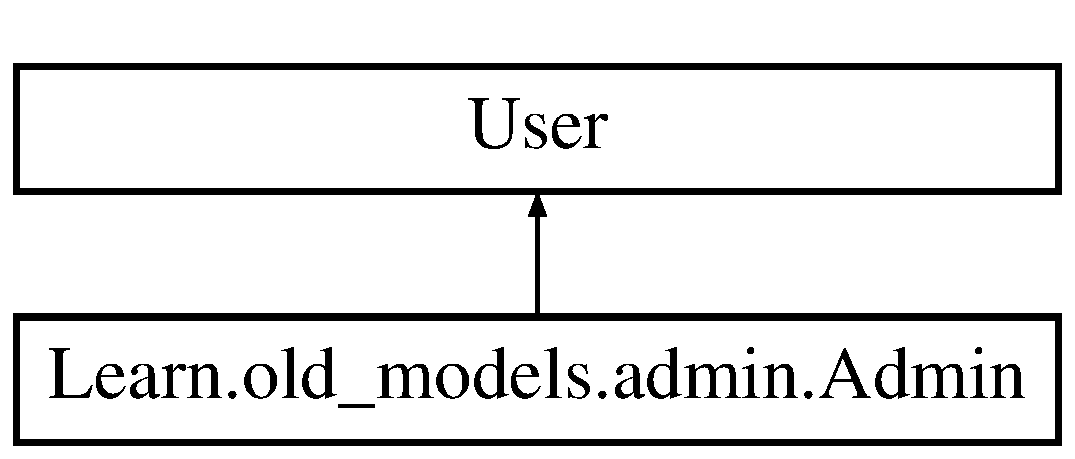
\includegraphics[height=2.000000cm]{class_learn_1_1old__models_1_1admin_1_1_admin}
\end{center}
\end{figure}
\subsection*{Classes}
\begin{DoxyCompactItemize}
\item 
class \hyperlink{class_learn_1_1old__models_1_1admin_1_1_admin_1_1_meta}{Meta}
\end{DoxyCompactItemize}
\subsection*{Static Public Attributes}
\begin{DoxyCompactItemize}
\item 
\hypertarget{class_learn_1_1old__models_1_1admin_1_1_admin_ad42fa652657a6cfb6a23167381e304fa}{tuple {\bfseries profession} models.\-Char\-Field(max\-\_\-length=50)}\label{class_learn_1_1old__models_1_1admin_1_1_admin_ad42fa652657a6cfb6a23167381e304fa}

\end{DoxyCompactItemize}


The documentation for this class was generated from the following file\-:\begin{DoxyCompactItemize}
\item 
/\-Users/\-Charlie/\-Documents/\-Aptana Studio 3 Workspace/\-C\-M2301-\/9/\-C\-M2301/\-Learn/old\-\_\-models/admin.\-py\end{DoxyCompactItemize}

\hypertarget{class_learn_1_1models_1_1_answer}{\section{Learn.\-models.\-Answer Class Reference}
\label{class_learn_1_1models_1_1_answer}\index{Learn.\-models.\-Answer@{Learn.\-models.\-Answer}}
}


An instance of the \hyperlink{class_learn_1_1models_1_1_answer}{Answer} class will hold text associated with an answer, and whether or not the answer is correct or not.  


Inheritance diagram for Learn.\-models.\-Answer\-:\begin{figure}[H]
\begin{center}
\leavevmode
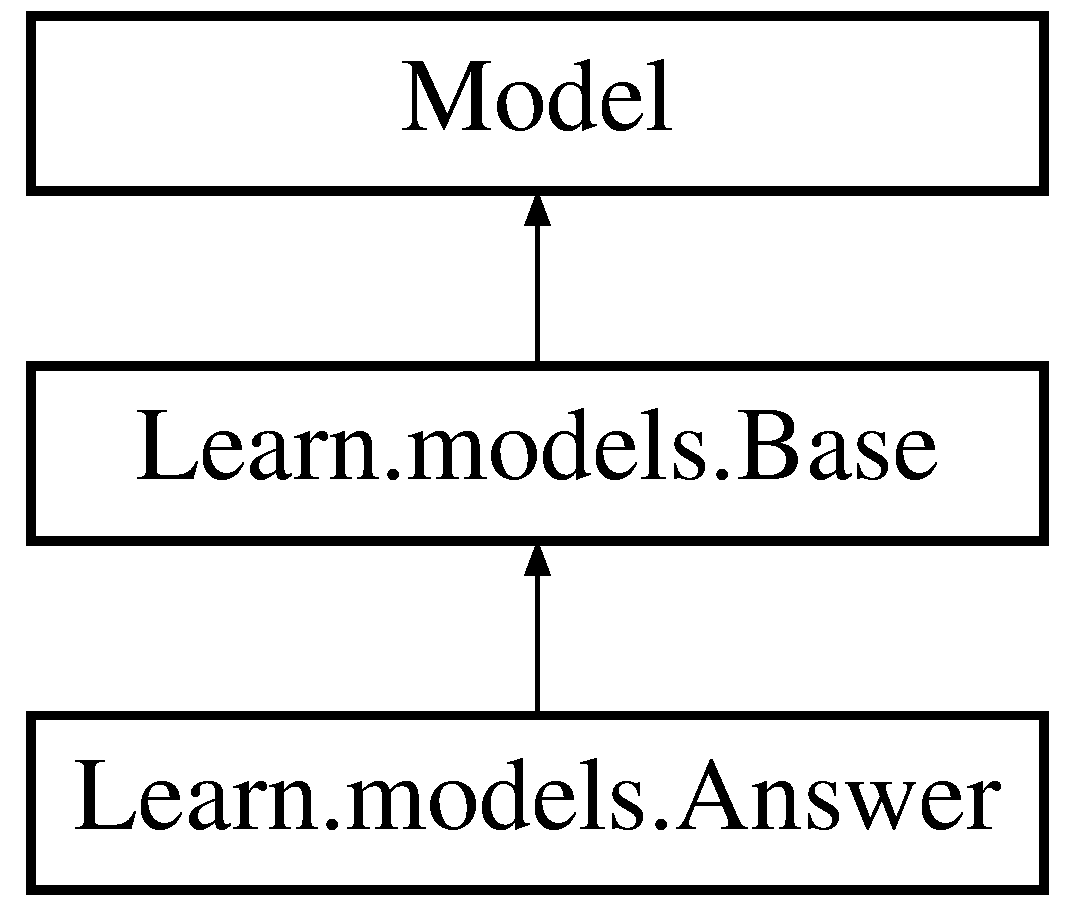
\includegraphics[height=3.000000cm]{class_learn_1_1models_1_1_answer}
\end{center}
\end{figure}
\subsection*{Static Public Attributes}
\begin{DoxyCompactItemize}
\item 
\hypertarget{class_learn_1_1models_1_1_answer_ac98b555cd170b3623cca09ecfa9d932b}{tuple {\bfseries content} models.\-Char\-Field(max\-\_\-length=250)}\label{class_learn_1_1models_1_1_answer_ac98b555cd170b3623cca09ecfa9d932b}

\item 
\hypertarget{class_learn_1_1models_1_1_answer_a0ec1628ee2d08f161cc25a82eea8ebb6}{tuple {\bfseries correct} models.\-Boolean\-Field()}\label{class_learn_1_1models_1_1_answer_a0ec1628ee2d08f161cc25a82eea8ebb6}

\item 
\hypertarget{class_learn_1_1models_1_1_answer_aa1194d87ee2fdbced15a5b551cf5e364}{tuple {\bfseries question} models.\-Foreign\-Key(\hyperlink{class_learn_1_1models_1_1_question}{Question})}\label{class_learn_1_1models_1_1_answer_aa1194d87ee2fdbced15a5b551cf5e364}

\end{DoxyCompactItemize}
\subsection*{Additional Inherited Members}


\subsection{Detailed Description}
An instance of the \hyperlink{class_learn_1_1models_1_1_answer}{Answer} class will hold text associated with an answer, and whether or not the answer is correct or not. 

The documentation for this class was generated from the following file\-:\begin{DoxyCompactItemize}
\item 
/\-Users/\-Charlie/\-Documents/\-Aptana Studio 3 Workspace/\-C\-M2301-\/9/\-C\-M2301/\-Learn/models.\-py\end{DoxyCompactItemize}

\hypertarget{class_learn_1_1models_1_1_attachment}{\section{Learn.\-models.\-Attachment Class Reference}
\label{class_learn_1_1models_1_1_attachment}\index{Learn.\-models.\-Attachment@{Learn.\-models.\-Attachment}}
}


An \hyperlink{class_learn_1_1models_1_1_attachment}{Attachment} is a collection of revisions.  


Inheritance diagram for Learn.\-models.\-Attachment\-:\begin{figure}[H]
\begin{center}
\leavevmode
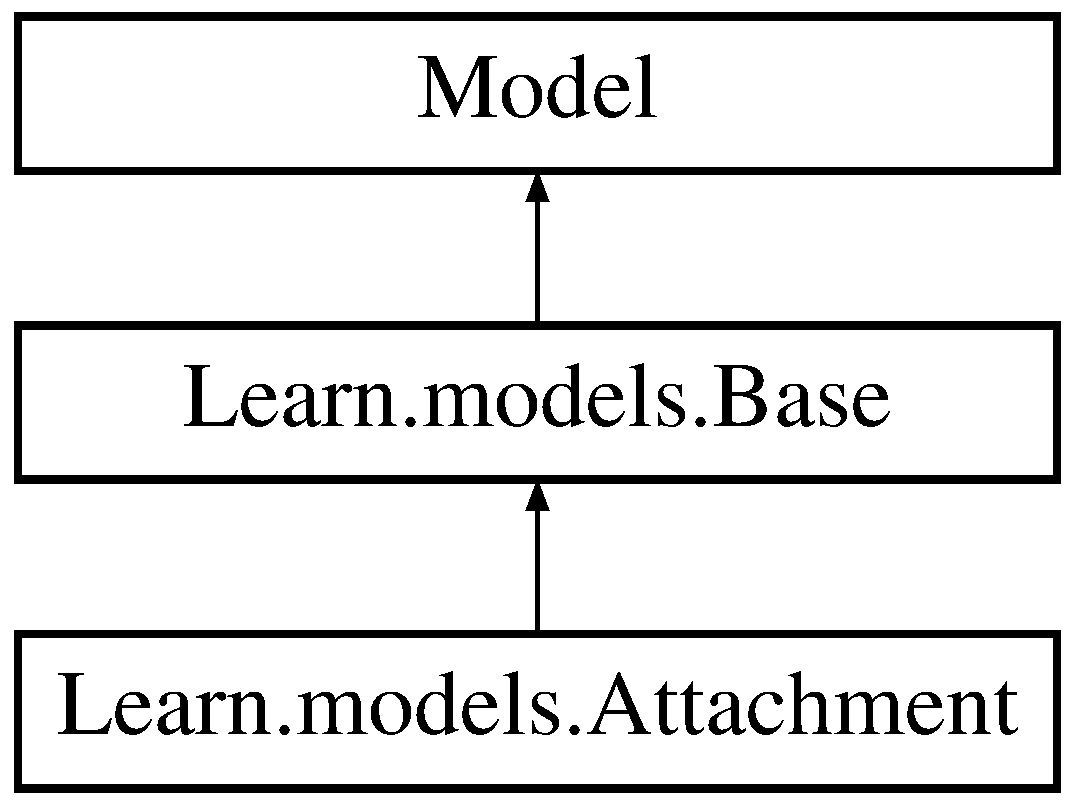
\includegraphics[height=3.000000cm]{class_learn_1_1models_1_1_attachment}
\end{center}
\end{figure}
\subsection*{Public Member Functions}
\begin{DoxyCompactItemize}
\item 
def \hyperlink{class_learn_1_1models_1_1_attachment_ad4529524ec5ff145986650657ee7a6fc}{get\-\_\-total\-\_\-size}
\begin{DoxyCompactList}\small\item\em Returns the total size used of all revisions in the \hyperlink{class_learn_1_1models_1_1_attachment}{Attachment} object. \end{DoxyCompactList}\item 
def \hyperlink{class_learn_1_1models_1_1_attachment_a022020821925beeb6da12429a75887e0}{remove\-\_\-revision}
\begin{DoxyCompactList}\small\item\em Removes the revision from the attachment with the specified uuid. \end{DoxyCompactList}\item 
\hypertarget{class_learn_1_1models_1_1_attachment_aee9d2a2edad4cd28e20720ab3b0242d4}{def \hyperlink{class_learn_1_1models_1_1_attachment_aee9d2a2edad4cd28e20720ab3b0242d4}{purge\-\_\-revisions}}\label{class_learn_1_1models_1_1_attachment_aee9d2a2edad4cd28e20720ab3b0242d4}

\begin{DoxyCompactList}\small\item\em Purges all Revisions but the most recent in the \hyperlink{class_learn_1_1models_1_1_attachment}{Attachment} object. \end{DoxyCompactList}\item 
def \hyperlink{class_learn_1_1models_1_1_attachment_a69cb6737bc80199fd2e79ab1a725f05e}{get\-\_\-all\-\_\-revisions}
\begin{DoxyCompactList}\small\item\em Returns an ordered List of revisions for the \hyperlink{class_learn_1_1models_1_1_attachment}{Attachment} based on time uploaded. \end{DoxyCompactList}\item 
def \hyperlink{class_learn_1_1models_1_1_attachment_a72fddbf30122110730c771f20b8a5714}{add\-\_\-revision}
\begin{DoxyCompactList}\small\item\em Adds the supplied \hyperlink{class_learn_1_1models_1_1_revision}{Revision} object to the \hyperlink{class_learn_1_1models_1_1_attachment}{Attachment} with current timestamp. \end{DoxyCompactList}\end{DoxyCompactItemize}
\subsection*{Static Public Attributes}
\begin{DoxyCompactItemize}
\item 
\hypertarget{class_learn_1_1models_1_1_attachment_a723dbad6b742dab4b2d86727cc281a9b}{tuple \hyperlink{class_learn_1_1models_1_1_attachment_a723dbad6b742dab4b2d86727cc281a9b}{title} models.\-Char\-Field(max\-\_\-length=50)}\label{class_learn_1_1models_1_1_attachment_a723dbad6b742dab4b2d86727cc281a9b}

\begin{DoxyCompactList}\small\item\em The title of the \hyperlink{class_learn_1_1models_1_1_attachment}{Attachment}. \end{DoxyCompactList}\item 
\hypertarget{class_learn_1_1models_1_1_attachment_a11126d7e4c4fde7af6b59962062cd2d0}{tuple \hyperlink{class_learn_1_1models_1_1_attachment_a11126d7e4c4fde7af6b59962062cd2d0}{file\-\_\-name} models.\-Char\-Field(max\-\_\-length=50)}\label{class_learn_1_1models_1_1_attachment_a11126d7e4c4fde7af6b59962062cd2d0}

\begin{DoxyCompactList}\small\item\em The file name e.\-g file.\-pdf. \end{DoxyCompactList}\item 
\hypertarget{class_learn_1_1models_1_1_attachment_acaf786996f915dbf370add35783e6194}{tuple \hyperlink{class_learn_1_1models_1_1_attachment_acaf786996f915dbf370add35783e6194}{description} models.\-Char\-Field(max\-\_\-length=250)}\label{class_learn_1_1models_1_1_attachment_acaf786996f915dbf370add35783e6194}

\begin{DoxyCompactList}\small\item\em The description of the \hyperlink{class_learn_1_1models_1_1_attachment}{Attachment}. \end{DoxyCompactList}\item 
tuple \hyperlink{class_learn_1_1models_1_1_attachment_a56f0ed9e935cf0f479db45afa52779a3}{owner} models.\-Foreign\-Key(\hyperlink{class_learn_1_1models_1_1_user}{User})
\begin{DoxyCompactList}\small\item\em The \hyperlink{class_learn_1_1models_1_1_user}{User} owning the \hyperlink{class_learn_1_1models_1_1_attachment}{Attachment}, usually the uploader. \end{DoxyCompactList}\end{DoxyCompactItemize}


\subsection{Detailed Description}
An \hyperlink{class_learn_1_1models_1_1_attachment}{Attachment} is a collection of revisions. 

\hyperlink{class_learn_1_1models_1_1_attachment}{Attachment} objects can be used to derive a full file revision history, and retrieve the original version of the file 

\subsection{Member Function Documentation}
\hypertarget{class_learn_1_1models_1_1_attachment_a72fddbf30122110730c771f20b8a5714}{\index{Learn\-::models\-::\-Attachment@{Learn\-::models\-::\-Attachment}!add\-\_\-revision@{add\-\_\-revision}}
\index{add\-\_\-revision@{add\-\_\-revision}!Learn::models::Attachment@{Learn\-::models\-::\-Attachment}}
\subsubsection[{add\-\_\-revision}]{\setlength{\rightskip}{0pt plus 5cm}def Learn.\-models.\-Attachment.\-add\-\_\-revision (
\begin{DoxyParamCaption}
\item[{}]{self, }
\item[{}]{revision}
\end{DoxyParamCaption}
)}}\label{class_learn_1_1models_1_1_attachment_a72fddbf30122110730c771f20b8a5714}


Adds the supplied \hyperlink{class_learn_1_1models_1_1_revision}{Revision} object to the \hyperlink{class_learn_1_1models_1_1_attachment}{Attachment} with current timestamp. 


\begin{DoxyParams}{Parameters}
{\em \hyperlink{class_learn_1_1models_1_1_revision}{Revision}} & The \hyperlink{class_learn_1_1models_1_1_revision}{Revision} object to add to the \hyperlink{class_learn_1_1models_1_1_attachment}{Attachment} \\
\hline
\end{DoxyParams}

\begin{DoxyExceptions}{Exceptions}
{\em Attachment\-Exception} & If \hyperlink{class_learn_1_1models_1_1_revision}{Revision} file type is invalid. \\
\hline
\end{DoxyExceptions}
\hypertarget{class_learn_1_1models_1_1_attachment_a69cb6737bc80199fd2e79ab1a725f05e}{\index{Learn\-::models\-::\-Attachment@{Learn\-::models\-::\-Attachment}!get\-\_\-all\-\_\-revisions@{get\-\_\-all\-\_\-revisions}}
\index{get\-\_\-all\-\_\-revisions@{get\-\_\-all\-\_\-revisions}!Learn::models::Attachment@{Learn\-::models\-::\-Attachment}}
\subsubsection[{get\-\_\-all\-\_\-revisions}]{\setlength{\rightskip}{0pt plus 5cm}def Learn.\-models.\-Attachment.\-get\-\_\-all\-\_\-revisions (
\begin{DoxyParamCaption}
\item[{}]{self}
\end{DoxyParamCaption}
)}}\label{class_learn_1_1models_1_1_attachment_a69cb6737bc80199fd2e79ab1a725f05e}


Returns an ordered List of revisions for the \hyperlink{class_learn_1_1models_1_1_attachment}{Attachment} based on time uploaded. 

\begin{DoxyReturn}{Returns}
List Returns a list of all Revisions sorted descending order. 
\end{DoxyReturn}
\hypertarget{class_learn_1_1models_1_1_attachment_ad4529524ec5ff145986650657ee7a6fc}{\index{Learn\-::models\-::\-Attachment@{Learn\-::models\-::\-Attachment}!get\-\_\-total\-\_\-size@{get\-\_\-total\-\_\-size}}
\index{get\-\_\-total\-\_\-size@{get\-\_\-total\-\_\-size}!Learn::models::Attachment@{Learn\-::models\-::\-Attachment}}
\subsubsection[{get\-\_\-total\-\_\-size}]{\setlength{\rightskip}{0pt plus 5cm}def Learn.\-models.\-Attachment.\-get\-\_\-total\-\_\-size (
\begin{DoxyParamCaption}
\item[{}]{self}
\end{DoxyParamCaption}
)}}\label{class_learn_1_1models_1_1_attachment_ad4529524ec5ff145986650657ee7a6fc}


Returns the total size used of all revisions in the \hyperlink{class_learn_1_1models_1_1_attachment}{Attachment} object. 

\begin{DoxyReturn}{Returns}
\-: Float A float of the total size in Kb 
\end{DoxyReturn}
\hypertarget{class_learn_1_1models_1_1_attachment_a022020821925beeb6da12429a75887e0}{\index{Learn\-::models\-::\-Attachment@{Learn\-::models\-::\-Attachment}!remove\-\_\-revision@{remove\-\_\-revision}}
\index{remove\-\_\-revision@{remove\-\_\-revision}!Learn::models::Attachment@{Learn\-::models\-::\-Attachment}}
\subsubsection[{remove\-\_\-revision}]{\setlength{\rightskip}{0pt plus 5cm}def Learn.\-models.\-Attachment.\-remove\-\_\-revision (
\begin{DoxyParamCaption}
\item[{}]{self, }
\item[{}]{revision\-\_\-uuid}
\end{DoxyParamCaption}
)}}\label{class_learn_1_1models_1_1_attachment_a022020821925beeb6da12429a75887e0}


Removes the revision from the attachment with the specified uuid. 


\begin{DoxyParams}{Parameters}
{\em U\-U\-I\-D} & The uuid of the revision to be purged. \\
\hline
\end{DoxyParams}
\begin{DoxyReturn}{Returns}
\hyperlink{class_learn_1_1models_1_1_revision}{Revision} The \hyperlink{class_learn_1_1models_1_1_revision}{Revision} object removed. 
\end{DoxyReturn}


\subsection{Member Data Documentation}
\hypertarget{class_learn_1_1models_1_1_attachment_a56f0ed9e935cf0f479db45afa52779a3}{\index{Learn\-::models\-::\-Attachment@{Learn\-::models\-::\-Attachment}!owner@{owner}}
\index{owner@{owner}!Learn::models::Attachment@{Learn\-::models\-::\-Attachment}}
\subsubsection[{owner}]{\setlength{\rightskip}{0pt plus 5cm}tuple Learn.\-models.\-Attachment.\-owner models.\-Foreign\-Key({\bf User})\hspace{0.3cm}{\ttfamily [static]}}}\label{class_learn_1_1models_1_1_attachment_a56f0ed9e935cf0f479db45afa52779a3}


The \hyperlink{class_learn_1_1models_1_1_user}{User} owning the \hyperlink{class_learn_1_1models_1_1_attachment}{Attachment}, usually the uploader. 



The documentation for this class was generated from the following file\-:\begin{DoxyCompactItemize}
\item 
/\-Users/\-Charlie/\-Documents/\-Aptana Studio 3 Workspace/\-C\-M2301-\/9/\-C\-M2301/\-Learn/models.\-py\end{DoxyCompactItemize}

\hypertarget{class_learn_1_1models_1_1_base}{\section{Learn.\-models.\-Base Class Reference}
\label{class_learn_1_1models_1_1_base}\index{Learn.\-models.\-Base@{Learn.\-models.\-Base}}
}


\hyperlink{class_learn_1_1models_1_1_base}{Base} class containing common properties and methods for models.  


Inheritance diagram for Learn.\-models.\-Base\-:\begin{figure}[H]
\begin{center}
\leavevmode
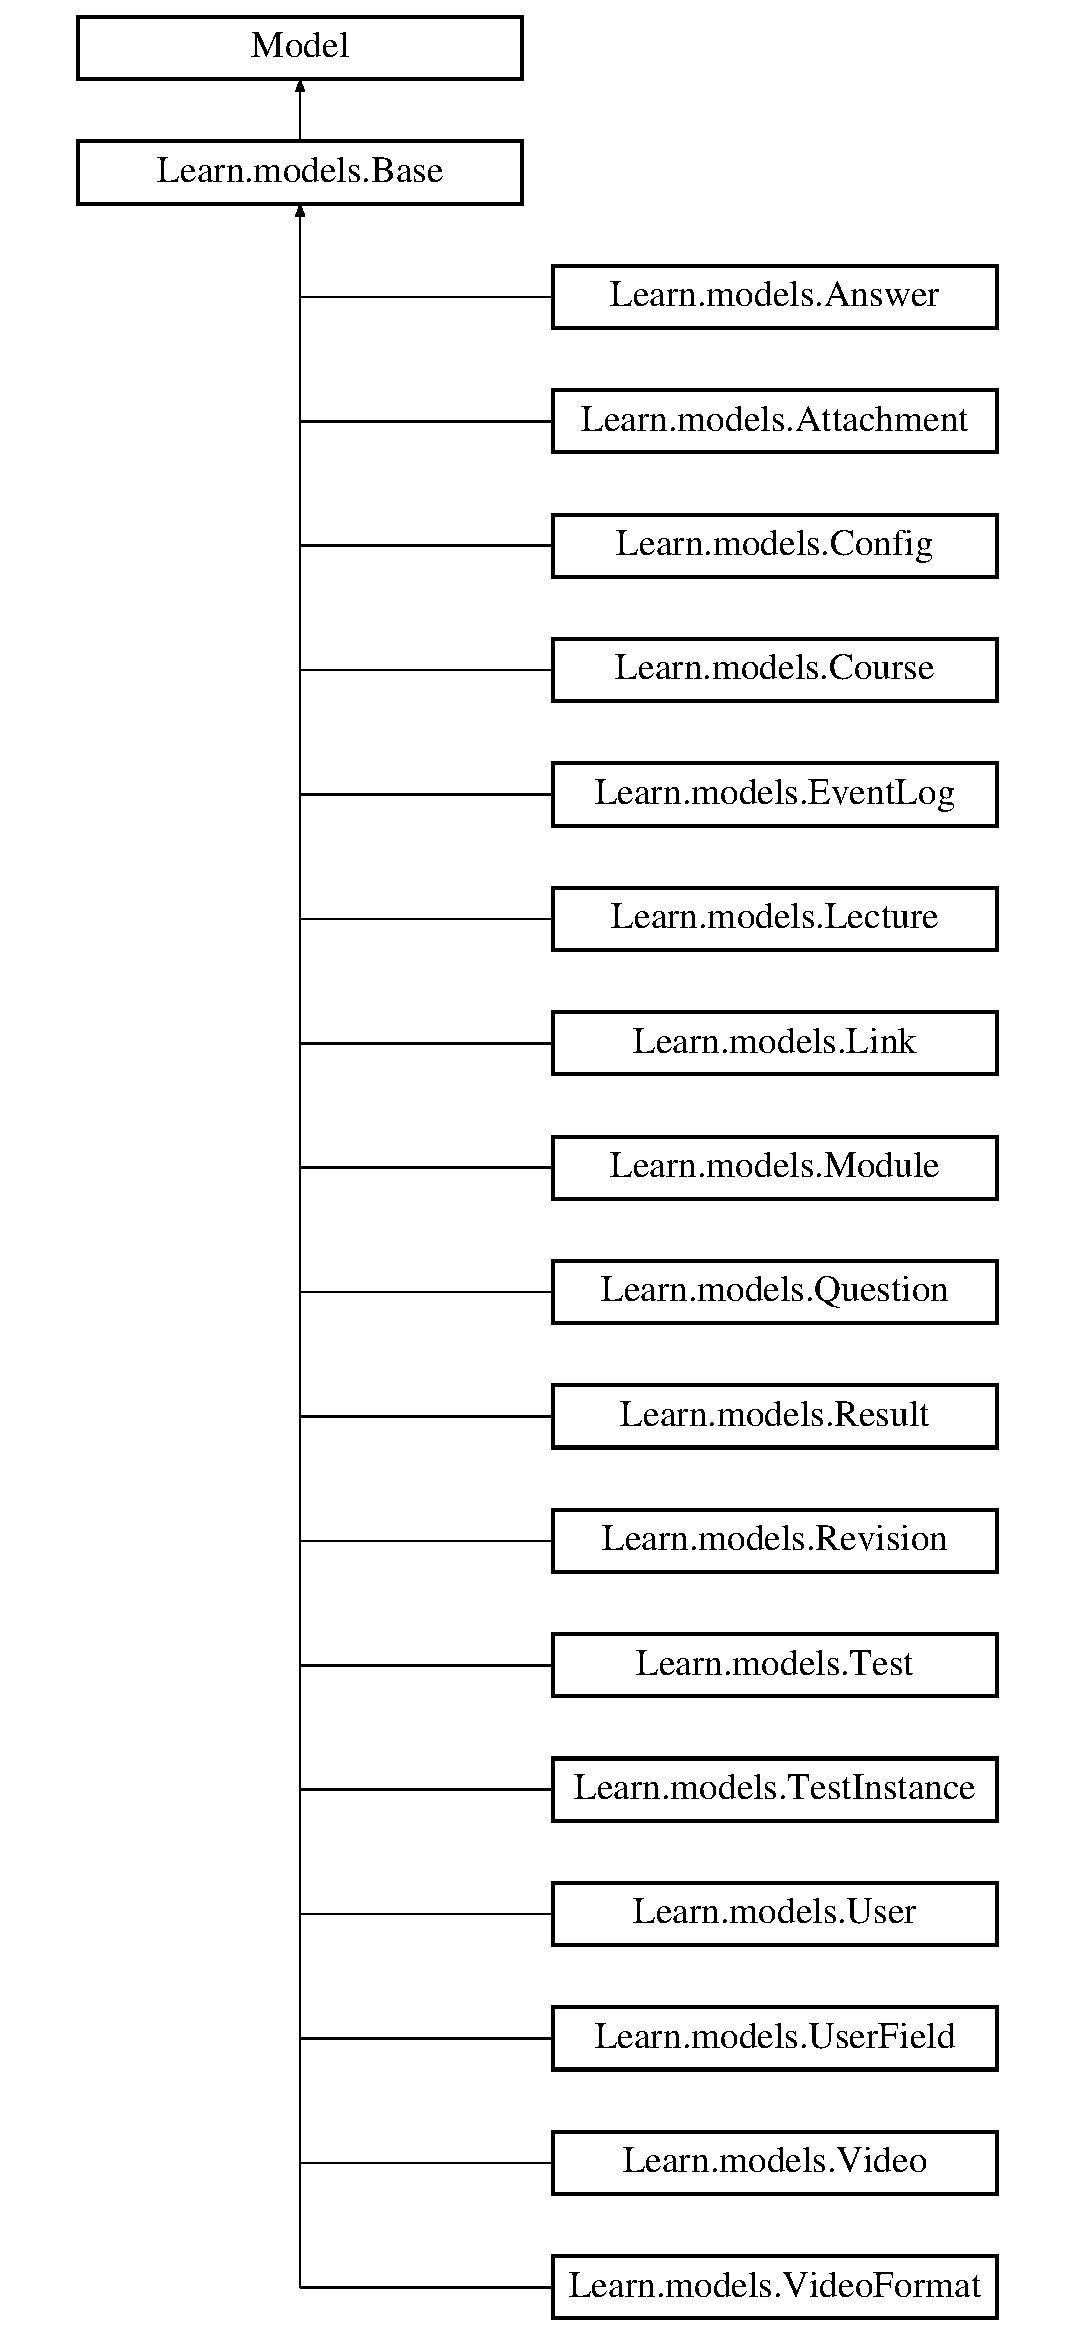
\includegraphics[height=12.000000cm]{class_learn_1_1models_1_1_base}
\end{center}
\end{figure}
\subsection*{Public Member Functions}
\begin{DoxyCompactItemize}
\item 
\hypertarget{class_learn_1_1models_1_1_base_a0674466843add52eb684b61bc487ddb6}{def \hyperlink{class_learn_1_1models_1_1_base_a0674466843add52eb684b61bc487ddb6}{save}}\label{class_learn_1_1models_1_1_base_a0674466843add52eb684b61bc487ddb6}

\begin{DoxyCompactList}\small\item\em Overrides the django.\-model.\-save() method to add a random U\-U\-I\-D to new objects before they are persisted to the D\-B. \end{DoxyCompactList}\end{DoxyCompactItemize}
\subsection*{Static Public Attributes}
\begin{DoxyCompactItemize}
\item 
\hypertarget{class_learn_1_1models_1_1_base_a7913a1f50c9ad34a1e217ea8ab5497db}{tuple \hyperlink{class_learn_1_1models_1_1_base_a7913a1f50c9ad34a1e217ea8ab5497db}{uuid} models.\-Char\-Field(max\-\_\-length=36, primary\-\_\-key=True)}\label{class_learn_1_1models_1_1_base_a7913a1f50c9ad34a1e217ea8ab5497db}

\begin{DoxyCompactList}\small\item\em U\-U\-I\-D of the object, as String. \end{DoxyCompactList}\end{DoxyCompactItemize}


\subsection{Detailed Description}
\hyperlink{class_learn_1_1models_1_1_base}{Base} class containing common properties and methods for models. 

All models will extend this class. 

The documentation for this class was generated from the following file\-:\begin{DoxyCompactItemize}
\item 
/\-Users/\-Charlie/\-Documents/\-Aptana Studio 3 Workspace/\-C\-M2301-\/9/\-C\-M2301/\-Learn/models.\-py\end{DoxyCompactItemize}

\hypertarget{class_learn_1_1models_1_1_config}{\section{Learn.\-models.\-Config Class Reference}
\label{class_learn_1_1models_1_1_config}\index{Learn.\-models.\-Config@{Learn.\-models.\-Config}}
}


Contains configuration and preferences for the system.  


Inheritance diagram for Learn.\-models.\-Config\-:\begin{figure}[H]
\begin{center}
\leavevmode
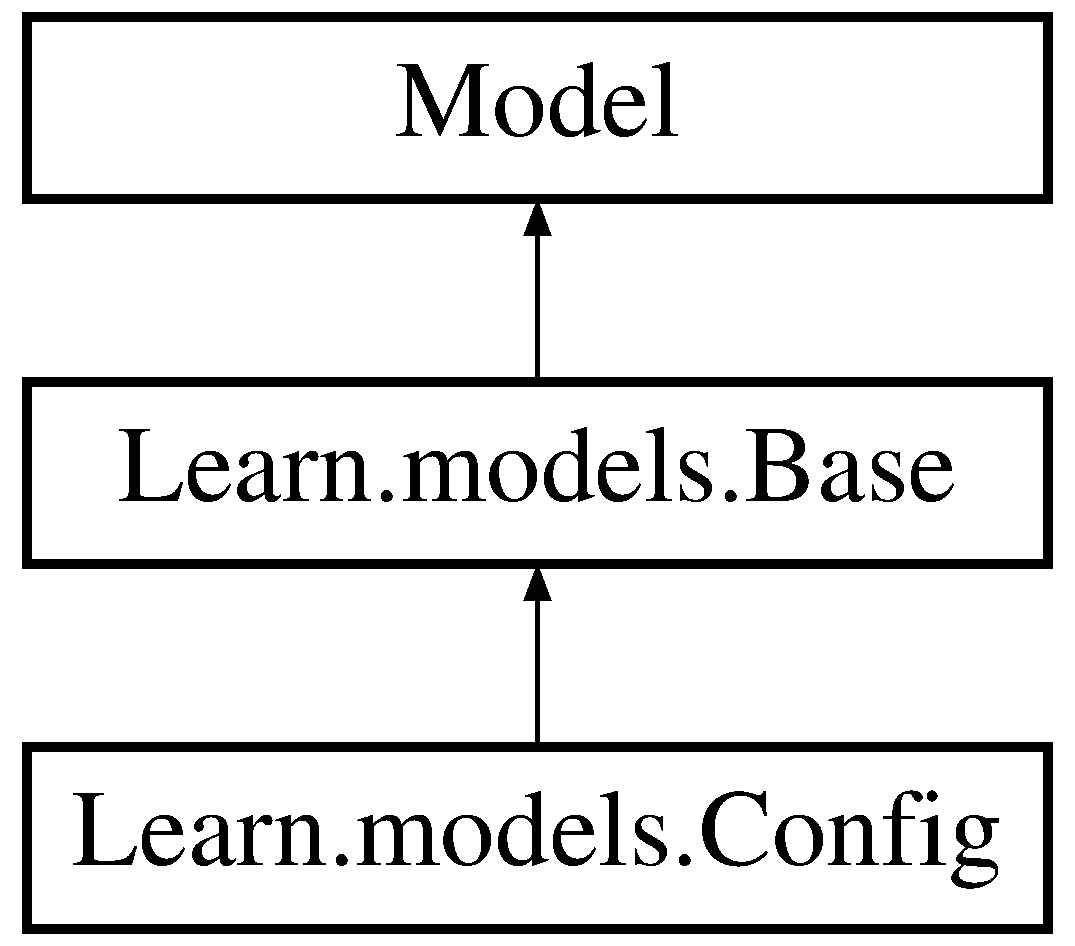
\includegraphics[height=3.000000cm]{class_learn_1_1models_1_1_config}
\end{center}
\end{figure}
\subsection*{Static Public Attributes}
\begin{DoxyCompactItemize}
\item 
\hypertarget{class_learn_1_1models_1_1_config_a14464f0683bf2c56133324c7849430d9}{tuple {\bfseries key} models.\-Char\-Field(max\-\_\-length=250)}\label{class_learn_1_1models_1_1_config_a14464f0683bf2c56133324c7849430d9}

\item 
\hypertarget{class_learn_1_1models_1_1_config_a37e7b20ea410084253f7153c9927aee0}{tuple {\bfseries data\-\_\-type} models.\-Char\-Field(max\-\_\-length=10)}\label{class_learn_1_1models_1_1_config_a37e7b20ea410084253f7153c9927aee0}

\item 
\hypertarget{class_learn_1_1models_1_1_config_a6a5401b43266f147e0f0b112749531c9}{tuple {\bfseries value} models.\-Text\-Field()}\label{class_learn_1_1models_1_1_config_a6a5401b43266f147e0f0b112749531c9}

\end{DoxyCompactItemize}
\subsection*{Additional Inherited Members}


\subsection{Detailed Description}
Contains configuration and preferences for the system. 

The documentation for this class was generated from the following file\-:\begin{DoxyCompactItemize}
\item 
/\-Users/\-Charlie/\-Documents/\-Aptana Studio 3 Workspace/\-C\-M2301-\/9/\-C\-M2301/\-Learn/models.\-py\end{DoxyCompactItemize}

\hypertarget{class_learn_1_1models_1_1_course}{\section{Learn.\-models.\-Course Class Reference}
\label{class_learn_1_1models_1_1_course}\index{Learn.\-models.\-Course@{Learn.\-models.\-Course}}
}


A course represents a top level definition of a degree, they are a collection of modules.  


Inheritance diagram for Learn.\-models.\-Course\-:\begin{figure}[H]
\begin{center}
\leavevmode
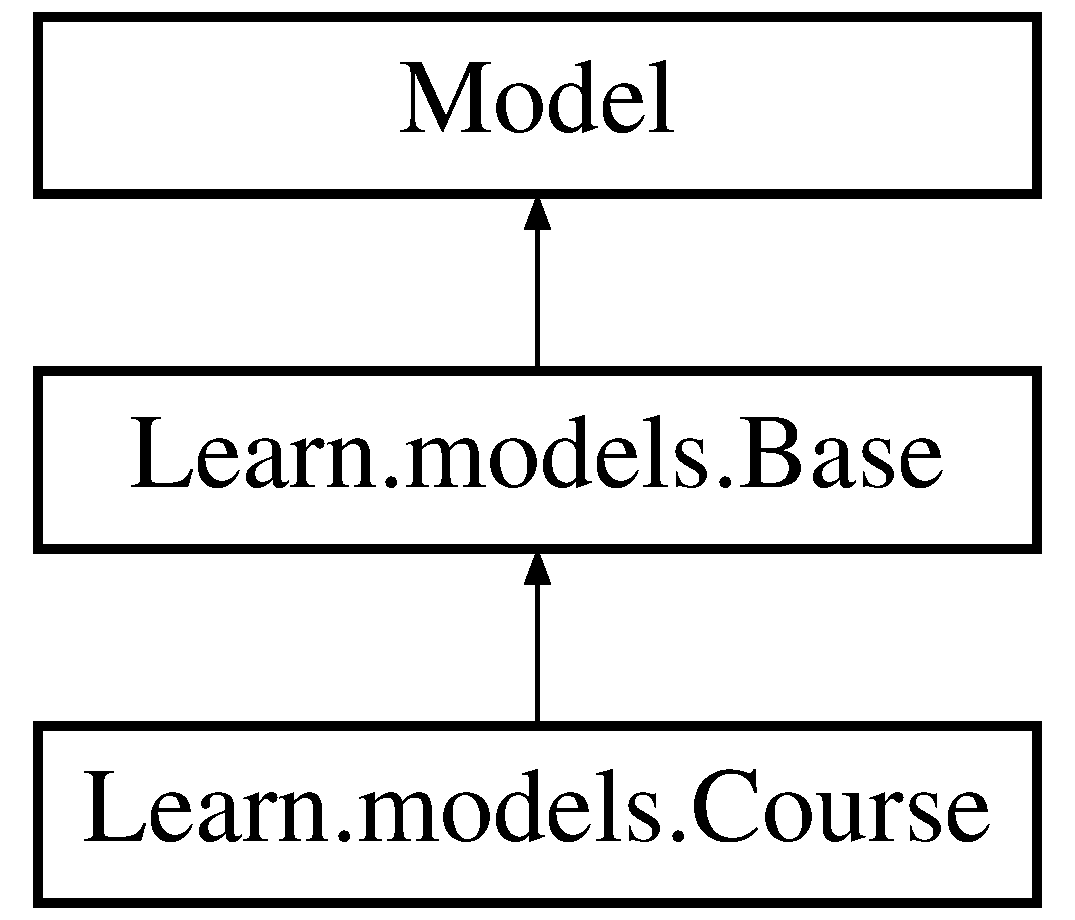
\includegraphics[height=3.000000cm]{class_learn_1_1models_1_1_course}
\end{center}
\end{figure}
\subsection*{Static Public Attributes}
\begin{DoxyCompactItemize}
\item 
\hypertarget{class_learn_1_1models_1_1_course_a5624ee47d76cd8a673dca4ba09814d4a}{tuple {\bfseries title} models.\-Char\-Field(max\-\_\-length=50)}\label{class_learn_1_1models_1_1_course_a5624ee47d76cd8a673dca4ba09814d4a}

\item 
\hypertarget{class_learn_1_1models_1_1_course_a3aa1038f195c829e34a0abf49249ad8c}{tuple {\bfseries code} models.\-Char\-Field(max\-\_\-length=50)}\label{class_learn_1_1models_1_1_course_a3aa1038f195c829e34a0abf49249ad8c}

\item 
\hypertarget{class_learn_1_1models_1_1_course_ac9321aac6e532207ee75d15e965bd95e}{tuple {\bfseries description} models.\-Text\-Field()}\label{class_learn_1_1models_1_1_course_ac9321aac6e532207ee75d15e965bd95e}

\item 
\hypertarget{class_learn_1_1models_1_1_course_ac24b32997392b177c57eb5546fe6d222}{tuple {\bfseries modules} models.\-Many\-To\-Many\-Field(\hyperlink{class_learn_1_1models_1_1_module}{Module})}\label{class_learn_1_1models_1_1_course_ac24b32997392b177c57eb5546fe6d222}

\item 
\hypertarget{class_learn_1_1models_1_1_course_a0ee169730bee73d15b4a4a8fb8640b97}{tuple {\bfseries attachments} models.\-Many\-To\-Many\-Field(\hyperlink{class_learn_1_1models_1_1_attachment}{Attachment})}\label{class_learn_1_1models_1_1_course_a0ee169730bee73d15b4a4a8fb8640b97}

\end{DoxyCompactItemize}
\subsection*{Additional Inherited Members}


\subsection{Detailed Description}
A course represents a top level definition of a degree, they are a collection of modules. 

The documentation for this class was generated from the following file\-:\begin{DoxyCompactItemize}
\item 
/\-Users/\-Charlie/\-Documents/\-Aptana Studio 3 Workspace/\-C\-M2301-\/9/\-C\-M2301/\-Learn/models.\-py\end{DoxyCompactItemize}

\hypertarget{classqueue_1_1_database}{\section{queue.\-Database Class Reference}
\label{classqueue_1_1_database}\index{queue.\-Database@{queue.\-Database}}
}
Inheritance diagram for queue.\-Database\-:\begin{figure}[H]
\begin{center}
\leavevmode
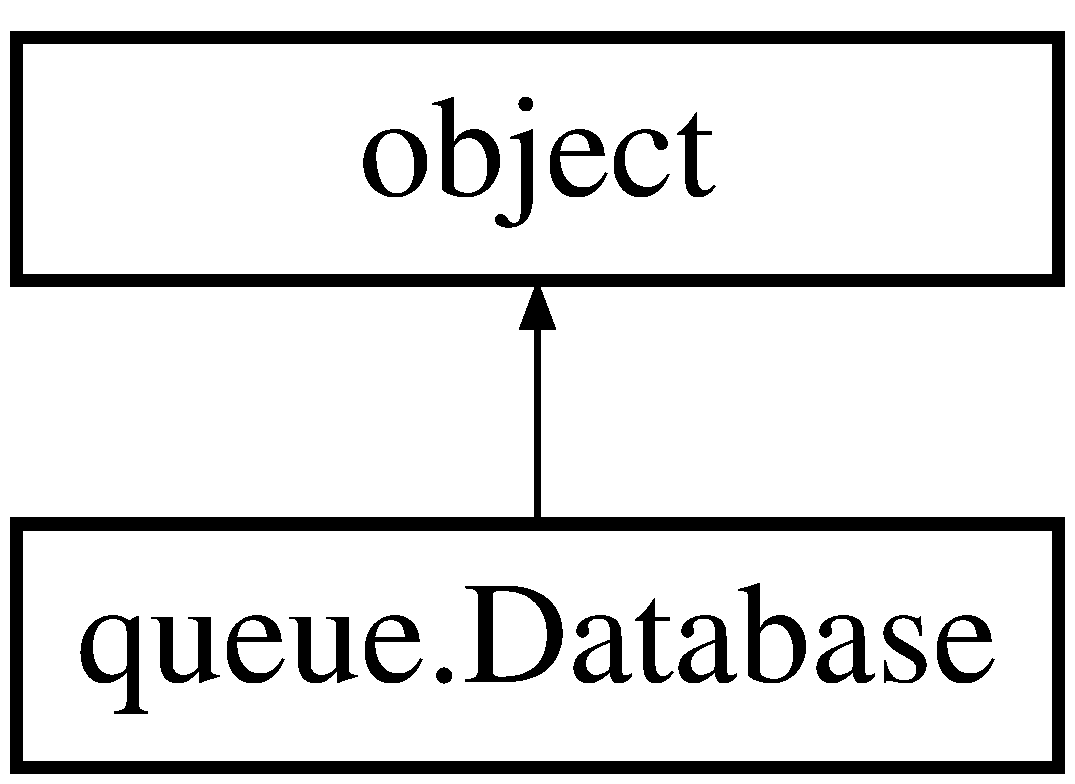
\includegraphics[height=2.000000cm]{classqueue_1_1_database}
\end{center}
\end{figure}
\subsection*{Public Member Functions}
\begin{DoxyCompactItemize}
\item 
\hypertarget{classqueue_1_1_database_a3714f51f945fc4721ff38eecc6c7a6a1}{def {\bfseries \-\_\-\-\_\-init\-\_\-\-\_\-}}\label{classqueue_1_1_database_a3714f51f945fc4721ff38eecc6c7a6a1}

\item 
\hypertarget{classqueue_1_1_database_a451ff193184fb189e2202e24c65d24b3}{def {\bfseries close}}\label{classqueue_1_1_database_a451ff193184fb189e2202e24c65d24b3}

\end{DoxyCompactItemize}
\subsection*{Static Public Attributes}
\begin{DoxyCompactItemize}
\item 
\hypertarget{classqueue_1_1_database_aff978a63409c521617345134d1b570f2}{string {\bfseries host} '127.\-0.\-0.\-1'}\label{classqueue_1_1_database_aff978a63409c521617345134d1b570f2}

\item 
\hypertarget{classqueue_1_1_database_a072fe6e42f893a197f16e5c6f3ca36d1}{string {\bfseries db} 'learn'}\label{classqueue_1_1_database_a072fe6e42f893a197f16e5c6f3ca36d1}

\item 
\hypertarget{classqueue_1_1_database_a5badc9d8c7bca15491073780b925a1b2}{string {\bfseries user} 'root'}\label{classqueue_1_1_database_a5badc9d8c7bca15491073780b925a1b2}

\item 
\hypertarget{classqueue_1_1_database_a0e936716a70aaddad972b9da66b7c1e9}{string {\bfseries psswd} ''}\label{classqueue_1_1_database_a0e936716a70aaddad972b9da66b7c1e9}

\item 
\hypertarget{classqueue_1_1_database_acbddd4806c9d47ec354cac2db47f8579}{{\bfseries con} None}\label{classqueue_1_1_database_acbddd4806c9d47ec354cac2db47f8579}

\item 
\hypertarget{classqueue_1_1_database_a3a5f44152f575fc32e7395ad1c6934a2}{{\bfseries cur} None}\label{classqueue_1_1_database_a3a5f44152f575fc32e7395ad1c6934a2}

\end{DoxyCompactItemize}


The documentation for this class was generated from the following file\-:\begin{DoxyCompactItemize}
\item 
/\-Users/\-Charlie/\-Documents/\-Aptana Studio 3 Workspace/\-C\-M2301-\/9/\-Server/queue.\-py\end{DoxyCompactItemize}

\hypertarget{class_learn_1_1models_1_1_event_log}{\section{Learn.\-models.\-Event\-Log Class Reference}
\label{class_learn_1_1models_1_1_event_log}\index{Learn.\-models.\-Event\-Log@{Learn.\-models.\-Event\-Log}}
}


Handles the storing of events in the log.  


Inheritance diagram for Learn.\-models.\-Event\-Log\-:\begin{figure}[H]
\begin{center}
\leavevmode
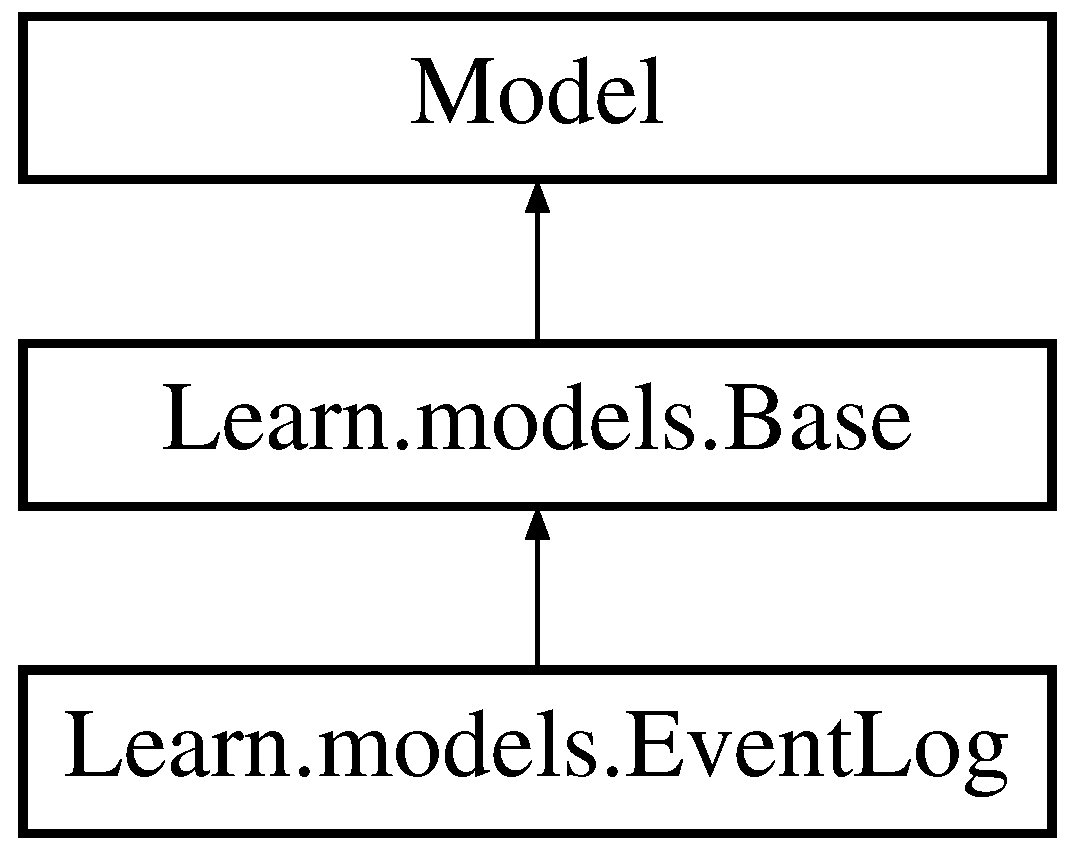
\includegraphics[height=3.000000cm]{class_learn_1_1models_1_1_event_log}
\end{center}
\end{figure}
\subsection*{Static Public Attributes}
\begin{DoxyCompactItemize}
\item 
\hypertarget{class_learn_1_1models_1_1_event_log_a59131c0acdcef88ad1a4c9bbe9b2dc07}{tuple {\bfseries event\-\_\-uuid} models.\-Char\-Field(max\-\_\-length=36)}\label{class_learn_1_1models_1_1_event_log_a59131c0acdcef88ad1a4c9bbe9b2dc07}

\item 
\hypertarget{class_learn_1_1models_1_1_event_log_a39076637215a65f0f9d523fa6b92e1e2}{tuple {\bfseries event\-\_\-type} models.\-Char\-Field(max\-\_\-length=50)}\label{class_learn_1_1models_1_1_event_log_a39076637215a65f0f9d523fa6b92e1e2}

\item 
\hypertarget{class_learn_1_1models_1_1_event_log_a9a9f44d173484578035963651e369573}{tuple {\bfseries severity} models.\-Char\-Field(max\-\_\-length=50)}\label{class_learn_1_1models_1_1_event_log_a9a9f44d173484578035963651e369573}

\item 
\hypertarget{class_learn_1_1models_1_1_event_log_af1e823d59a06eed2e4d7b7fdf131d0dc}{tuple {\bfseries content} models.\-Text\-Field()}\label{class_learn_1_1models_1_1_event_log_af1e823d59a06eed2e4d7b7fdf131d0dc}

\item 
\hypertarget{class_learn_1_1models_1_1_event_log_a588a2a950da0fdc2c6de2365b9ac07ef}{tuple {\bfseries timestamp} models.\-Date\-Time\-Field()}\label{class_learn_1_1models_1_1_event_log_a588a2a950da0fdc2c6de2365b9ac07ef}

\end{DoxyCompactItemize}
\subsection*{Additional Inherited Members}


\subsection{Detailed Description}
Handles the storing of events in the log. 

The documentation for this class was generated from the following file\-:\begin{DoxyCompactItemize}
\item 
/\-Users/\-Charlie/\-Documents/\-Aptana Studio 3 Workspace/\-C\-M2301-\/9/\-C\-M2301/\-Learn/models.\-py\end{DoxyCompactItemize}

\hypertarget{class_learn_1_1models_1_1_lecture}{\section{Learn.\-models.\-Lecture Class Reference}
\label{class_learn_1_1models_1_1_lecture}\index{Learn.\-models.\-Lecture@{Learn.\-models.\-Lecture}}
}


Represents a lecture within a module.  


Inheritance diagram for Learn.\-models.\-Lecture\-:\begin{figure}[H]
\begin{center}
\leavevmode
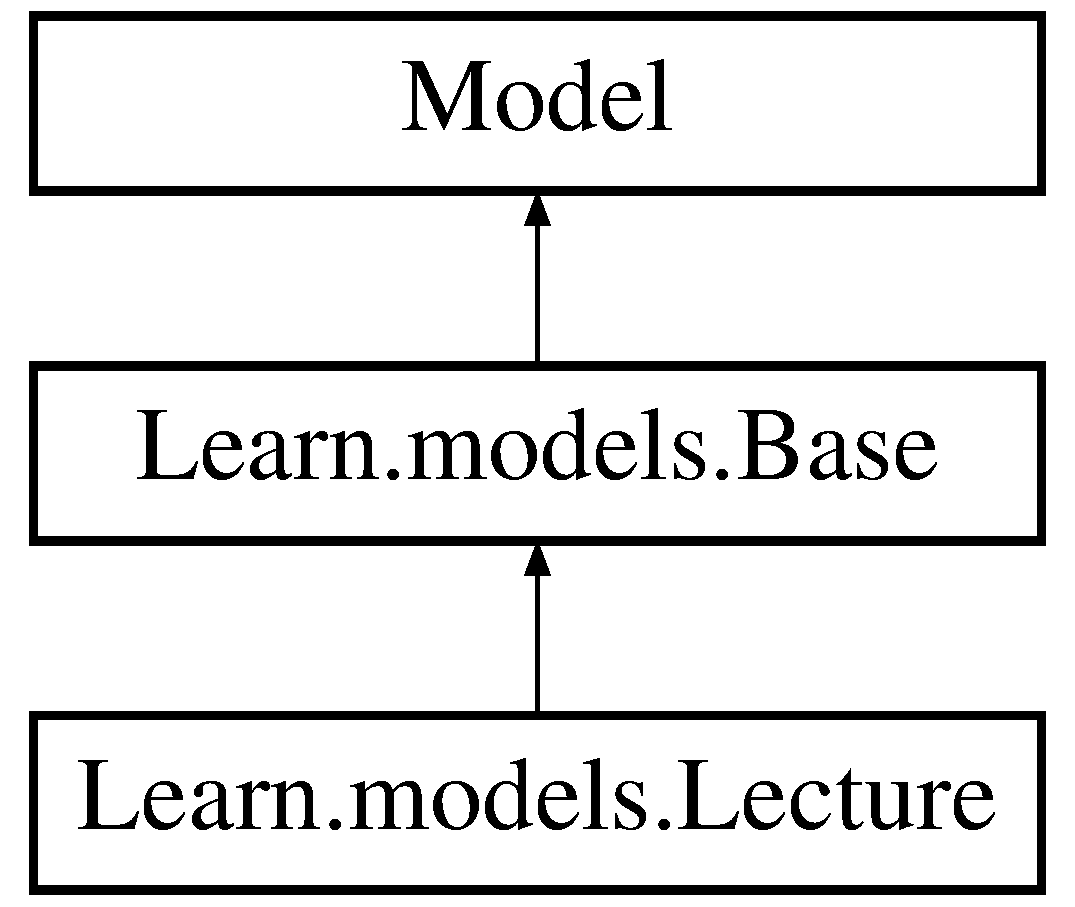
\includegraphics[height=3.000000cm]{class_learn_1_1models_1_1_lecture}
\end{center}
\end{figure}
\subsection*{Static Public Attributes}
\begin{DoxyCompactItemize}
\item 
\hypertarget{class_learn_1_1models_1_1_lecture_ab3b7fb800f000c80f1110480c7d35933}{tuple {\bfseries title} models.\-Char\-Field(max\-\_\-length=50)}\label{class_learn_1_1models_1_1_lecture_ab3b7fb800f000c80f1110480c7d35933}

\item 
\hypertarget{class_learn_1_1models_1_1_lecture_ac19083c89180f81e3f20147b2107159c}{tuple {\bfseries videos} models.\-Many\-To\-Many\-Field(\hyperlink{class_learn_1_1models_1_1_video}{Video})}\label{class_learn_1_1models_1_1_lecture_ac19083c89180f81e3f20147b2107159c}

\item 
\hypertarget{class_learn_1_1models_1_1_lecture_af75889e8ad3a0a94e9391e61542be336}{tuple {\bfseries attachments} models.\-Many\-To\-Many\-Field(\hyperlink{class_learn_1_1models_1_1_attachment}{Attachment})}\label{class_learn_1_1models_1_1_lecture_af75889e8ad3a0a94e9391e61542be336}

\item 
\hypertarget{class_learn_1_1models_1_1_lecture_a69edbeec19d878a65e0d872ec116b78b}{tuple {\bfseries valid\-From} models.\-Date\-Field()}\label{class_learn_1_1models_1_1_lecture_a69edbeec19d878a65e0d872ec116b78b}

\item 
\hypertarget{class_learn_1_1models_1_1_lecture_ae466aaba7429a70e009fcea6e94e3f02}{tuple {\bfseries valid\-To} models.\-Date\-Field()}\label{class_learn_1_1models_1_1_lecture_ae466aaba7429a70e009fcea6e94e3f02}

\item 
\hypertarget{class_learn_1_1models_1_1_lecture_ae895aa3e48283081eb38066335feecd6}{tuple {\bfseries visible} models.\-Boolean\-Field(default=True)}\label{class_learn_1_1models_1_1_lecture_ae895aa3e48283081eb38066335feecd6}

\item 
\hypertarget{class_learn_1_1models_1_1_lecture_a6dcf95b7e3c94bc30a5d131ffc80dc30}{tuple {\bfseries links} models.\-Many\-To\-Many\-Field(\hyperlink{class_learn_1_1models_1_1_link}{Link})}\label{class_learn_1_1models_1_1_lecture_a6dcf95b7e3c94bc30a5d131ffc80dc30}

\item 
\hypertarget{class_learn_1_1models_1_1_lecture_ac7c762a2effa5f31cbc8e3cda5ab31f8}{tuple {\bfseries lecturers} models.\-Many\-To\-Many\-Field(\hyperlink{class_learn_1_1models_1_1_user}{User})}\label{class_learn_1_1models_1_1_lecture_ac7c762a2effa5f31cbc8e3cda5ab31f8}

\end{DoxyCompactItemize}
\subsection*{Additional Inherited Members}


\subsection{Detailed Description}
Represents a lecture within a module. 

Contains details about an individual lecture \& references to lecture content (Videos, Attachments and \hyperlink{class_learn_1_1models_1_1_lecture}{Lecture} Notes). 

The documentation for this class was generated from the following file\-:\begin{DoxyCompactItemize}
\item 
/\-Users/\-Charlie/\-Documents/\-Aptana Studio 3 Workspace/\-C\-M2301-\/9/\-C\-M2301/\-Learn/models.\-py\end{DoxyCompactItemize}

\hypertarget{class_learn_1_1old__models_1_1lecture_1_1_lecture}{\section{Learn.\-old\-\_\-models.\-lecture.\-Lecture Class Reference}
\label{class_learn_1_1old__models_1_1lecture_1_1_lecture}\index{Learn.\-old\-\_\-models.\-lecture.\-Lecture@{Learn.\-old\-\_\-models.\-lecture.\-Lecture}}
}
Inheritance diagram for Learn.\-old\-\_\-models.\-lecture.\-Lecture\-:\begin{figure}[H]
\begin{center}
\leavevmode
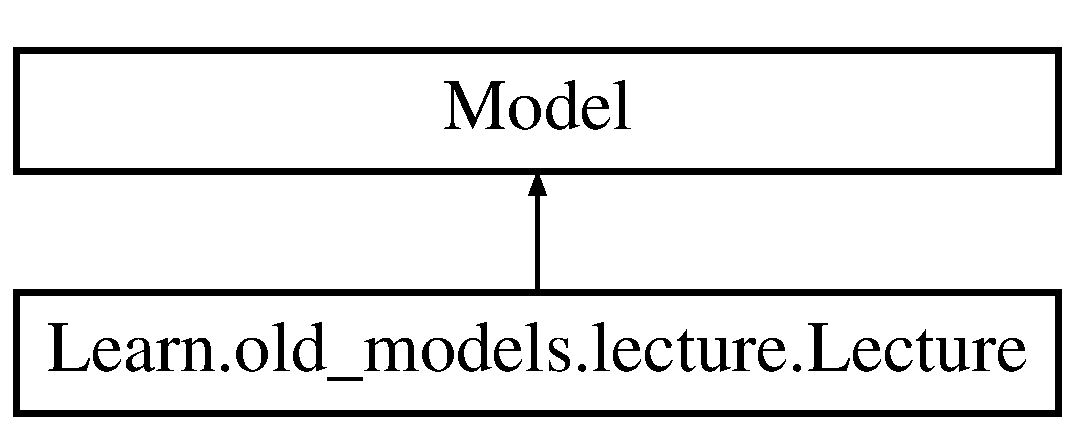
\includegraphics[height=2.000000cm]{class_learn_1_1old__models_1_1lecture_1_1_lecture}
\end{center}
\end{figure}
\subsection*{Classes}
\begin{DoxyCompactItemize}
\item 
class \hyperlink{class_learn_1_1old__models_1_1lecture_1_1_lecture_1_1_meta}{Meta}
\end{DoxyCompactItemize}
\subsection*{Public Member Functions}
\begin{DoxyCompactItemize}
\item 
\hypertarget{class_learn_1_1old__models_1_1lecture_1_1_lecture_a16803c9b0489d53e43de7c03ef5635d8}{def {\bfseries \-\_\-\-\_\-init\-\_\-\-\_\-}}\label{class_learn_1_1old__models_1_1lecture_1_1_lecture_a16803c9b0489d53e43de7c03ef5635d8}

\end{DoxyCompactItemize}
\subsection*{Public Attributes}
\begin{DoxyCompactItemize}
\item 
\hypertarget{class_learn_1_1old__models_1_1lecture_1_1_lecture_a366f435d7adb01ee95ecc79d319fef24}{{\bfseries uuid}}\label{class_learn_1_1old__models_1_1lecture_1_1_lecture_a366f435d7adb01ee95ecc79d319fef24}

\end{DoxyCompactItemize}
\subsection*{Static Public Attributes}
\begin{DoxyCompactItemize}
\item 
\hypertarget{class_learn_1_1old__models_1_1lecture_1_1_lecture_a0fe1bfb4370a4c4cd31150e893b76b89}{tuple {\bfseries uuid} models.\-Char\-Field(max\-\_\-length=36, primary\-\_\-key=True)}\label{class_learn_1_1old__models_1_1lecture_1_1_lecture_a0fe1bfb4370a4c4cd31150e893b76b89}

\item 
\hypertarget{class_learn_1_1old__models_1_1lecture_1_1_lecture_af8a037e83af9421629c045ecfa4411ca}{tuple {\bfseries title} models.\-Char\-Field(max\-\_\-length=100)}\label{class_learn_1_1old__models_1_1lecture_1_1_lecture_af8a037e83af9421629c045ecfa4411ca}

\item 
\hypertarget{class_learn_1_1old__models_1_1lecture_1_1_lecture_a0e7d2f600ceb875b40573b44e32d8de2}{tuple {\bfseries module} models.\-Char\-Field(max\-\_\-length=50)}\label{class_learn_1_1old__models_1_1lecture_1_1_lecture_a0e7d2f600ceb875b40573b44e32d8de2}

\item 
\hypertarget{class_learn_1_1old__models_1_1lecture_1_1_lecture_ad1bd86b9f846efc920bcef702f401575}{tuple {\bfseries videos} models.\-Char\-Field(max\-\_\-length=50)}\label{class_learn_1_1old__models_1_1lecture_1_1_lecture_ad1bd86b9f846efc920bcef702f401575}

\item 
\hypertarget{class_learn_1_1old__models_1_1lecture_1_1_lecture_ae23d7c625e9061602e171cd0ec39a748}{tuple {\bfseries attachments} models.\-Char\-Field(max\-\_\-length=50)}\label{class_learn_1_1old__models_1_1lecture_1_1_lecture_ae23d7c625e9061602e171cd0ec39a748}

\item 
\hypertarget{class_learn_1_1old__models_1_1lecture_1_1_lecture_a27c4fbb26f3f904948e470261339e437}{tuple {\bfseries visible} models.\-Boolean\-Field()}\label{class_learn_1_1old__models_1_1lecture_1_1_lecture_a27c4fbb26f3f904948e470261339e437}

\item 
\hypertarget{class_learn_1_1old__models_1_1lecture_1_1_lecture_aef2e743687f525490951c670637b6715}{tuple {\bfseries links} models.\-Char\-Field(max\-\_\-length=50)}\label{class_learn_1_1old__models_1_1lecture_1_1_lecture_aef2e743687f525490951c670637b6715}

\end{DoxyCompactItemize}


The documentation for this class was generated from the following file\-:\begin{DoxyCompactItemize}
\item 
/\-Users/\-Charlie/\-Documents/\-Aptana Studio 3 Workspace/\-C\-M2301-\/9/\-C\-M2301/\-Learn/old\-\_\-models/lecture.\-py\end{DoxyCompactItemize}

\hypertarget{class_learn_1_1old__models_1_1lecturer_1_1_lecturer}{\section{Learn.\-old\-\_\-models.\-lecturer.\-Lecturer Class Reference}
\label{class_learn_1_1old__models_1_1lecturer_1_1_lecturer}\index{Learn.\-old\-\_\-models.\-lecturer.\-Lecturer@{Learn.\-old\-\_\-models.\-lecturer.\-Lecturer}}
}
Inheritance diagram for Learn.\-old\-\_\-models.\-lecturer.\-Lecturer\-:\begin{figure}[H]
\begin{center}
\leavevmode
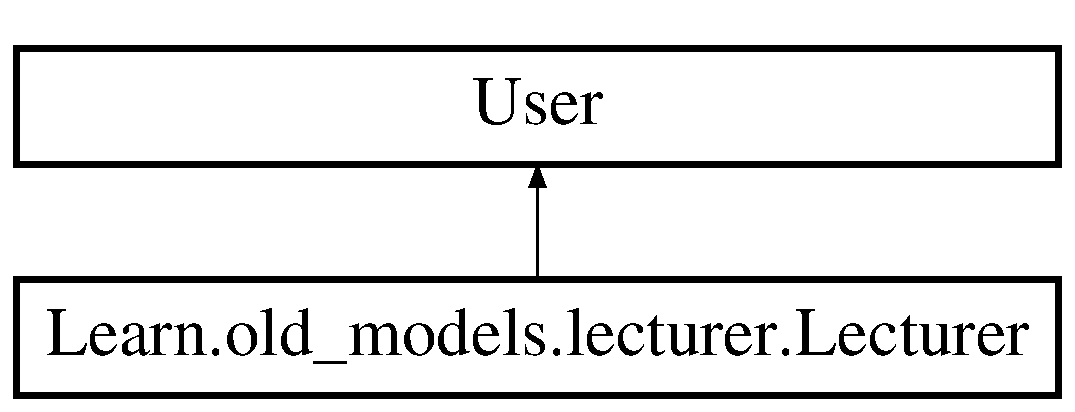
\includegraphics[height=2.000000cm]{class_learn_1_1old__models_1_1lecturer_1_1_lecturer}
\end{center}
\end{figure}
\subsection*{Classes}
\begin{DoxyCompactItemize}
\item 
class \hyperlink{class_learn_1_1old__models_1_1lecturer_1_1_lecturer_1_1_meta}{Meta}
\end{DoxyCompactItemize}
\subsection*{Static Public Attributes}
\begin{DoxyCompactItemize}
\item 
\hypertarget{class_learn_1_1old__models_1_1lecturer_1_1_lecturer_a63338f93b9f3be069e08addee1eda971}{tuple {\bfseries profession} models.\-Char\-Field(max\-\_\-length=100)}\label{class_learn_1_1old__models_1_1lecturer_1_1_lecturer_a63338f93b9f3be069e08addee1eda971}

\item 
\hypertarget{class_learn_1_1old__models_1_1lecturer_1_1_lecturer_a50734669b4b00936aede7e4bdc7225d0}{tuple {\bfseries lectures} models.\-Foreign\-Key(Lecture)}\label{class_learn_1_1old__models_1_1lecturer_1_1_lecturer_a50734669b4b00936aede7e4bdc7225d0}

\end{DoxyCompactItemize}


The documentation for this class was generated from the following file\-:\begin{DoxyCompactItemize}
\item 
/\-Users/\-Charlie/\-Documents/\-Aptana Studio 3 Workspace/\-C\-M2301-\/9/\-C\-M2301/\-Learn/old\-\_\-models/lecturer.\-py\end{DoxyCompactItemize}

\hypertarget{class_learn_1_1models_1_1_link}{\section{Learn.\-models.\-Link Class Reference}
\label{class_learn_1_1models_1_1_link}\index{Learn.\-models.\-Link@{Learn.\-models.\-Link}}
}


Holds to a resource.  


Inheritance diagram for Learn.\-models.\-Link\-:\begin{figure}[H]
\begin{center}
\leavevmode
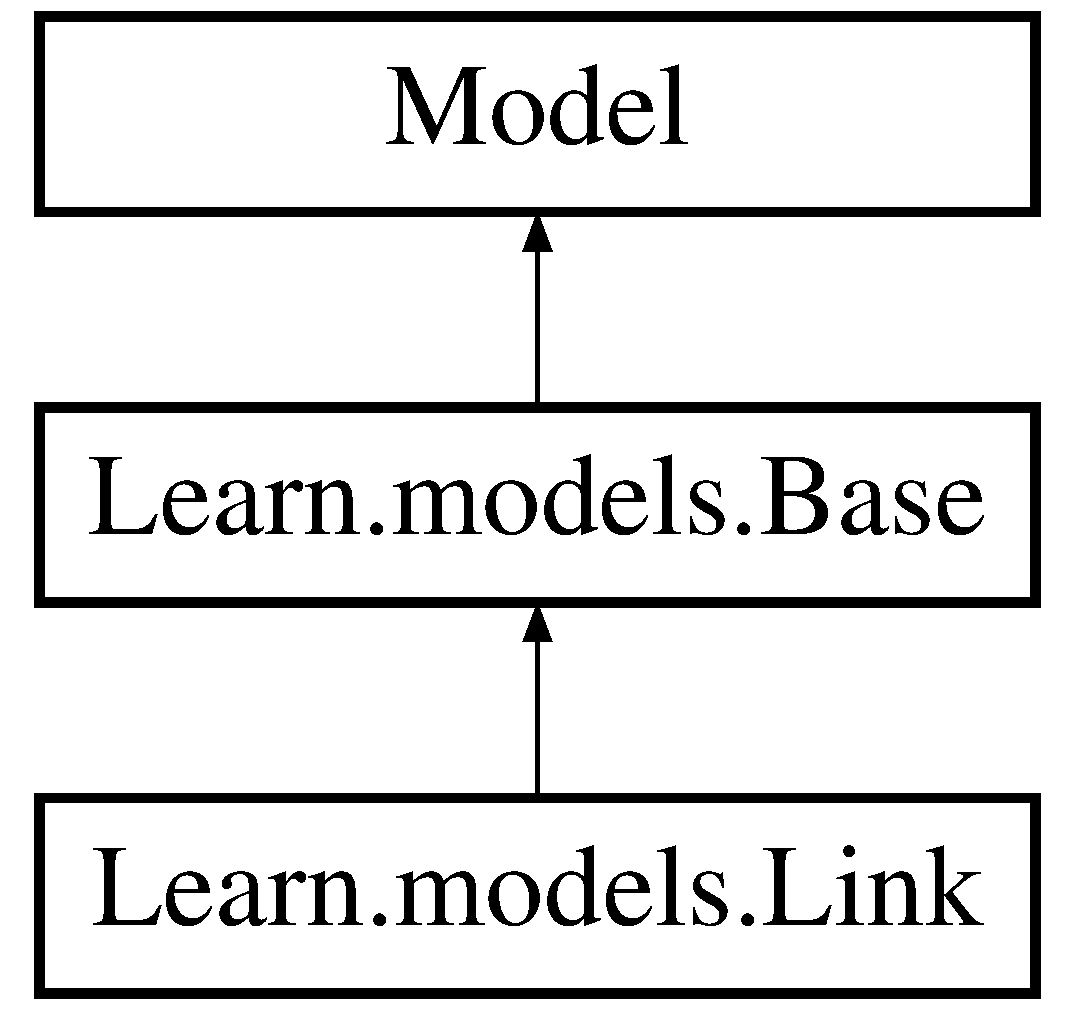
\includegraphics[height=3.000000cm]{class_learn_1_1models_1_1_link}
\end{center}
\end{figure}
\subsection*{Static Public Attributes}
\begin{DoxyCompactItemize}
\item 
\hypertarget{class_learn_1_1models_1_1_link_ae21cfe86a0aaeb6d3eeb01b695b74973}{tuple \hyperlink{class_learn_1_1models_1_1_link_ae21cfe86a0aaeb6d3eeb01b695b74973}{title} models.\-Char\-Field(max\-\_\-length=250)}\label{class_learn_1_1models_1_1_link_ae21cfe86a0aaeb6d3eeb01b695b74973}

\begin{DoxyCompactList}\small\item\em The title for the \hyperlink{class_learn_1_1models_1_1_link}{Link} story. \end{DoxyCompactList}\item 
\hypertarget{class_learn_1_1models_1_1_link_ab76a421b4eca1067173a38ff83ce8922}{tuple \hyperlink{class_learn_1_1models_1_1_link_ab76a421b4eca1067173a38ff83ce8922}{description} models.\-Text\-Field()}\label{class_learn_1_1models_1_1_link_ab76a421b4eca1067173a38ff83ce8922}

\begin{DoxyCompactList}\small\item\em The description of the \hyperlink{class_learn_1_1models_1_1_link}{Link}. \end{DoxyCompactList}\item 
\hypertarget{class_learn_1_1models_1_1_link_a03bc9e8cebd0340c75d15fd57fff99e1}{tuple \hyperlink{class_learn_1_1models_1_1_link_a03bc9e8cebd0340c75d15fd57fff99e1}{link} models.\-U\-R\-L\-Field(max\-\_\-length=250)}\label{class_learn_1_1models_1_1_link_a03bc9e8cebd0340c75d15fd57fff99e1}

\begin{DoxyCompactList}\small\item\em The \hyperlink{class_learn_1_1models_1_1_link}{Link} U\-Rl in string form. \end{DoxyCompactList}\end{DoxyCompactItemize}
\subsection*{Additional Inherited Members}


\subsection{Detailed Description}
Holds to a resource. 

Links can be added to many other Objects. 

The documentation for this class was generated from the following file\-:\begin{DoxyCompactItemize}
\item 
/\-Users/\-Charlie/\-Documents/\-Aptana Studio 3 Workspace/\-C\-M2301-\/9/\-C\-M2301/\-Learn/models.\-py\end{DoxyCompactItemize}

\hypertarget{class_learn_1_1old__models_1_1admin_1_1_admin_1_1_meta}{\section{Learn.\-old\-\_\-models.\-admin.\-Admin.\-Meta Class Reference}
\label{class_learn_1_1old__models_1_1admin_1_1_admin_1_1_meta}\index{Learn.\-old\-\_\-models.\-admin.\-Admin.\-Meta@{Learn.\-old\-\_\-models.\-admin.\-Admin.\-Meta}}
}
\subsection*{Static Public Attributes}
\begin{DoxyCompactItemize}
\item 
\hypertarget{class_learn_1_1old__models_1_1admin_1_1_admin_1_1_meta_a0de4f88834b8b773bb1581f19e87a4bd}{string {\bfseries app\-\_\-label} \char`\"{}Learn\char`\"{}}\label{class_learn_1_1old__models_1_1admin_1_1_admin_1_1_meta_a0de4f88834b8b773bb1581f19e87a4bd}

\end{DoxyCompactItemize}


The documentation for this class was generated from the following file\-:\begin{DoxyCompactItemize}
\item 
/\-Users/\-Charlie/\-Documents/\-Aptana Studio 3 Workspace/\-C\-M2301-\/9/\-C\-M2301/\-Learn/old\-\_\-models/admin.\-py\end{DoxyCompactItemize}

\hypertarget{class_learn_1_1old__models_1_1lecture_1_1_lecture_1_1_meta}{\section{Learn.\-old\-\_\-models.\-lecture.\-Lecture.\-Meta Class Reference}
\label{class_learn_1_1old__models_1_1lecture_1_1_lecture_1_1_meta}\index{Learn.\-old\-\_\-models.\-lecture.\-Lecture.\-Meta@{Learn.\-old\-\_\-models.\-lecture.\-Lecture.\-Meta}}
}
\subsection*{Static Public Attributes}
\begin{DoxyCompactItemize}
\item 
\hypertarget{class_learn_1_1old__models_1_1lecture_1_1_lecture_1_1_meta_ade4be4e3ca571b9115a7b92548c4faab}{string {\bfseries app\-\_\-label} \char`\"{}Learn\char`\"{}}\label{class_learn_1_1old__models_1_1lecture_1_1_lecture_1_1_meta_ade4be4e3ca571b9115a7b92548c4faab}

\end{DoxyCompactItemize}


The documentation for this class was generated from the following file\-:\begin{DoxyCompactItemize}
\item 
/\-Users/\-Charlie/\-Documents/\-Aptana Studio 3 Workspace/\-C\-M2301-\/9/\-C\-M2301/\-Learn/old\-\_\-models/lecture.\-py\end{DoxyCompactItemize}

\hypertarget{class_learn_1_1old__models_1_1lecturer_1_1_lecturer_1_1_meta}{\section{Learn.\-old\-\_\-models.\-lecturer.\-Lecturer.\-Meta Class Reference}
\label{class_learn_1_1old__models_1_1lecturer_1_1_lecturer_1_1_meta}\index{Learn.\-old\-\_\-models.\-lecturer.\-Lecturer.\-Meta@{Learn.\-old\-\_\-models.\-lecturer.\-Lecturer.\-Meta}}
}
\subsection*{Static Public Attributes}
\begin{DoxyCompactItemize}
\item 
\hypertarget{class_learn_1_1old__models_1_1lecturer_1_1_lecturer_1_1_meta_af686033849a880e4c71d95cb1b1555ac}{string {\bfseries app\-\_\-label} \char`\"{}Learn\char`\"{}}\label{class_learn_1_1old__models_1_1lecturer_1_1_lecturer_1_1_meta_af686033849a880e4c71d95cb1b1555ac}

\end{DoxyCompactItemize}


The documentation for this class was generated from the following file\-:\begin{DoxyCompactItemize}
\item 
/\-Users/\-Charlie/\-Documents/\-Aptana Studio 3 Workspace/\-C\-M2301-\/9/\-C\-M2301/\-Learn/old\-\_\-models/lecturer.\-py\end{DoxyCompactItemize}

\hypertarget{class_learn_1_1old__models_1_1queue_1_1_queue_1_1_meta}{\section{Learn.\-old\-\_\-models.\-queue.\-Queue.\-Meta Class Reference}
\label{class_learn_1_1old__models_1_1queue_1_1_queue_1_1_meta}\index{Learn.\-old\-\_\-models.\-queue.\-Queue.\-Meta@{Learn.\-old\-\_\-models.\-queue.\-Queue.\-Meta}}
}
\subsection*{Static Public Attributes}
\begin{DoxyCompactItemize}
\item 
\hypertarget{class_learn_1_1old__models_1_1queue_1_1_queue_1_1_meta_a203ff739d7c26be78545b3be4d07a070}{string {\bfseries app\-\_\-label} \char`\"{}Learn\char`\"{}}\label{class_learn_1_1old__models_1_1queue_1_1_queue_1_1_meta_a203ff739d7c26be78545b3be4d07a070}

\end{DoxyCompactItemize}


The documentation for this class was generated from the following file\-:\begin{DoxyCompactItemize}
\item 
/\-Users/\-Charlie/\-Documents/\-Aptana Studio 3 Workspace/\-C\-M2301-\/9/\-C\-M2301/\-Learn/old\-\_\-models/queue.\-py\end{DoxyCompactItemize}

\hypertarget{class_learn_1_1old__models_1_1student_1_1_student_1_1_meta}{\section{Learn.\-old\-\_\-models.\-student.\-Student.\-Meta Class Reference}
\label{class_learn_1_1old__models_1_1student_1_1_student_1_1_meta}\index{Learn.\-old\-\_\-models.\-student.\-Student.\-Meta@{Learn.\-old\-\_\-models.\-student.\-Student.\-Meta}}
}
\subsection*{Static Public Attributes}
\begin{DoxyCompactItemize}
\item 
\hypertarget{class_learn_1_1old__models_1_1student_1_1_student_1_1_meta_a7350cc4280e66a5535cd502c44743c92}{string {\bfseries app\-\_\-label} \char`\"{}Learn\char`\"{}}\label{class_learn_1_1old__models_1_1student_1_1_student_1_1_meta_a7350cc4280e66a5535cd502c44743c92}

\end{DoxyCompactItemize}


The documentation for this class was generated from the following file\-:\begin{DoxyCompactItemize}
\item 
/\-Users/\-Charlie/\-Documents/\-Aptana Studio 3 Workspace/\-C\-M2301-\/9/\-C\-M2301/\-Learn/old\-\_\-models/student.\-py\end{DoxyCompactItemize}

\hypertarget{class_learn_1_1old__models_1_1user_1_1_user_1_1_meta}{\section{Learn.\-old\-\_\-models.\-user.\-User.\-Meta Class Reference}
\label{class_learn_1_1old__models_1_1user_1_1_user_1_1_meta}\index{Learn.\-old\-\_\-models.\-user.\-User.\-Meta@{Learn.\-old\-\_\-models.\-user.\-User.\-Meta}}
}
\subsection*{Static Public Attributes}
\begin{DoxyCompactItemize}
\item 
\hypertarget{class_learn_1_1old__models_1_1user_1_1_user_1_1_meta_ac2af85f358931aa70076ec75a6e99e02}{string {\bfseries app\-\_\-label} \char`\"{}Learn\char`\"{}}\label{class_learn_1_1old__models_1_1user_1_1_user_1_1_meta_ac2af85f358931aa70076ec75a6e99e02}

\item 
\hypertarget{class_learn_1_1old__models_1_1user_1_1_user_1_1_meta_a293506bbccbb0669dbdfff32e18b5c7a}{{\bfseries abstract} True}\label{class_learn_1_1old__models_1_1user_1_1_user_1_1_meta_a293506bbccbb0669dbdfff32e18b5c7a}

\end{DoxyCompactItemize}


The documentation for this class was generated from the following file\-:\begin{DoxyCompactItemize}
\item 
/\-Users/\-Charlie/\-Documents/\-Aptana Studio 3 Workspace/\-C\-M2301-\/9/\-C\-M2301/\-Learn/old\-\_\-models/user.\-py\end{DoxyCompactItemize}

\hypertarget{class_learn_1_1models_1_1_module}{\section{Learn.\-models.\-Module Class Reference}
\label{class_learn_1_1models_1_1_module}\index{Learn.\-models.\-Module@{Learn.\-models.\-Module}}
}


A module belonging to a course.  


Inheritance diagram for Learn.\-models.\-Module\-:\begin{figure}[H]
\begin{center}
\leavevmode
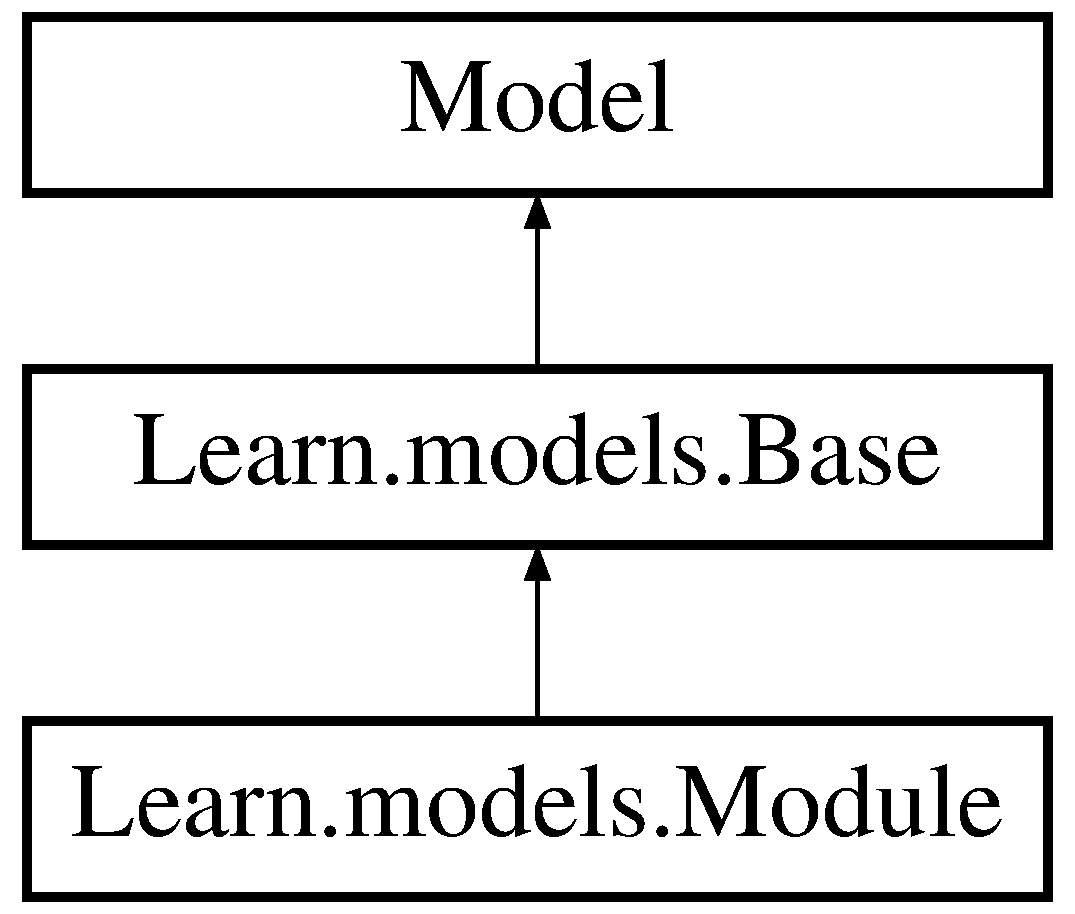
\includegraphics[height=3.000000cm]{class_learn_1_1models_1_1_module}
\end{center}
\end{figure}
\subsection*{Static Public Attributes}
\begin{DoxyCompactItemize}
\item 
\hypertarget{class_learn_1_1models_1_1_module_a6681a4334338d2b737625c6f9919d47c}{tuple {\bfseries title} models.\-Char\-Field(max\-\_\-length=100)}\label{class_learn_1_1models_1_1_module_a6681a4334338d2b737625c6f9919d47c}

\item 
\hypertarget{class_learn_1_1models_1_1_module_ab8669b2e30cc2503f2b9c046b69fbf81}{tuple {\bfseries module\-\_\-code} models.\-Char\-Field(max\-\_\-length=100)}\label{class_learn_1_1models_1_1_module_ab8669b2e30cc2503f2b9c046b69fbf81}

\item 
\hypertarget{class_learn_1_1models_1_1_module_a0c8e0fa400f13699981bc68b73530c9a}{tuple {\bfseries attachments} models.\-Many\-To\-Many\-Field(\hyperlink{class_learn_1_1models_1_1_attachment}{Attachment})}\label{class_learn_1_1models_1_1_module_a0c8e0fa400f13699981bc68b73530c9a}

\item 
\hypertarget{class_learn_1_1models_1_1_module_a360e290c667908a5b0a792f5517ba53b}{tuple {\bfseries lectures} models.\-Many\-To\-Many\-Field(\hyperlink{class_learn_1_1models_1_1_lecture}{Lecture})}\label{class_learn_1_1models_1_1_module_a360e290c667908a5b0a792f5517ba53b}

\end{DoxyCompactItemize}
\subsection*{Additional Inherited Members}


\subsection{Detailed Description}
A module belonging to a course. 

The documentation for this class was generated from the following file\-:\begin{DoxyCompactItemize}
\item 
/\-Users/\-Charlie/\-Documents/\-Aptana Studio 3 Workspace/\-C\-M2301-\/9/\-C\-M2301/\-Learn/models.\-py\end{DoxyCompactItemize}

\hypertarget{class_learn_1_1models_1_1_question}{\section{Learn.\-models.\-Question Class Reference}
\label{class_learn_1_1models_1_1_question}\index{Learn.\-models.\-Question@{Learn.\-models.\-Question}}
}


An instance of the \hyperlink{class_learn_1_1models_1_1_question}{Question} class will hold the question string with a List of answer objects that the user can pick.  


Inheritance diagram for Learn.\-models.\-Question\-:\begin{figure}[H]
\begin{center}
\leavevmode
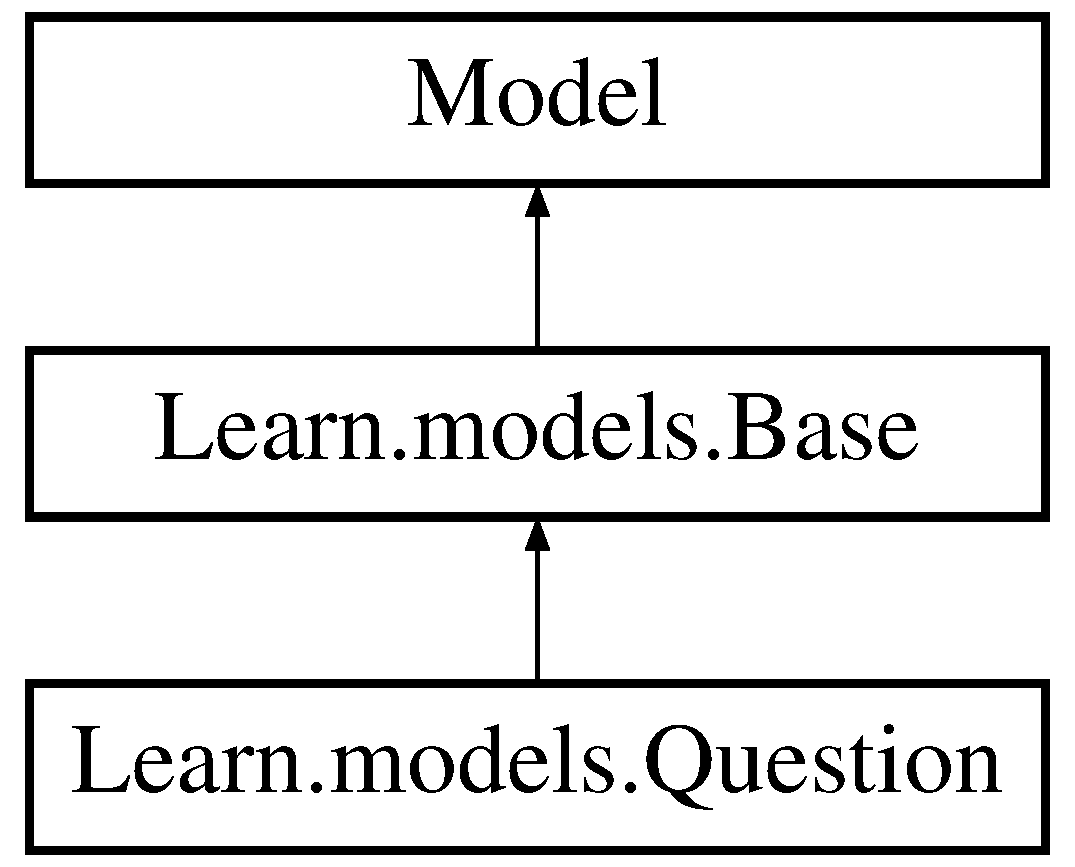
\includegraphics[height=3.000000cm]{class_learn_1_1models_1_1_question}
\end{center}
\end{figure}
\subsection*{Public Member Functions}
\begin{DoxyCompactItemize}
\item 
\hypertarget{class_learn_1_1models_1_1_question_a20099b8a66509aabc45c926eb1b8ab66}{def \hyperlink{class_learn_1_1models_1_1_question_a20099b8a66509aabc45c926eb1b8ab66}{get\-\_\-answers}}\label{class_learn_1_1models_1_1_question_a20099b8a66509aabc45c926eb1b8ab66}

\begin{DoxyCompactList}\small\item\em Returns the possible answers for the question. \end{DoxyCompactList}\item 
\hypertarget{class_learn_1_1models_1_1_question_a308fcf01d3db05841a842996789b2507}{def \hyperlink{class_learn_1_1models_1_1_question_a308fcf01d3db05841a842996789b2507}{get\-\_\-correct\-\_\-answer}}\label{class_learn_1_1models_1_1_question_a308fcf01d3db05841a842996789b2507}

\begin{DoxyCompactList}\small\item\em Returns the correct answer for the question. \end{DoxyCompactList}\end{DoxyCompactItemize}
\subsection*{Static Public Attributes}
\begin{DoxyCompactItemize}
\item 
\hypertarget{class_learn_1_1models_1_1_question_ad11386e06fa22f48129ec588d6caa491}{tuple {\bfseries content} models.\-Text\-Field()}\label{class_learn_1_1models_1_1_question_ad11386e06fa22f48129ec588d6caa491}

\item 
\hypertarget{class_learn_1_1models_1_1_question_aed186eae128695191043fc31e012b07e}{tuple {\bfseries type} models.\-Char\-Field(max\-\_\-length=40)}\label{class_learn_1_1models_1_1_question_aed186eae128695191043fc31e012b07e}

\end{DoxyCompactItemize}


\subsection{Detailed Description}
An instance of the \hyperlink{class_learn_1_1models_1_1_question}{Question} class will hold the question string with a List of answer objects that the user can pick. 

The documentation for this class was generated from the following file\-:\begin{DoxyCompactItemize}
\item 
/\-Users/\-Charlie/\-Documents/\-Aptana Studio 3 Workspace/\-C\-M2301-\/9/\-C\-M2301/\-Learn/models.\-py\end{DoxyCompactItemize}

\hypertarget{class_learn_1_1old__models_1_1queue_1_1_queue}{\section{Learn.\-old\-\_\-models.\-queue.\-Queue Class Reference}
\label{class_learn_1_1old__models_1_1queue_1_1_queue}\index{Learn.\-old\-\_\-models.\-queue.\-Queue@{Learn.\-old\-\_\-models.\-queue.\-Queue}}
}
Inheritance diagram for Learn.\-old\-\_\-models.\-queue.\-Queue\-:\begin{figure}[H]
\begin{center}
\leavevmode
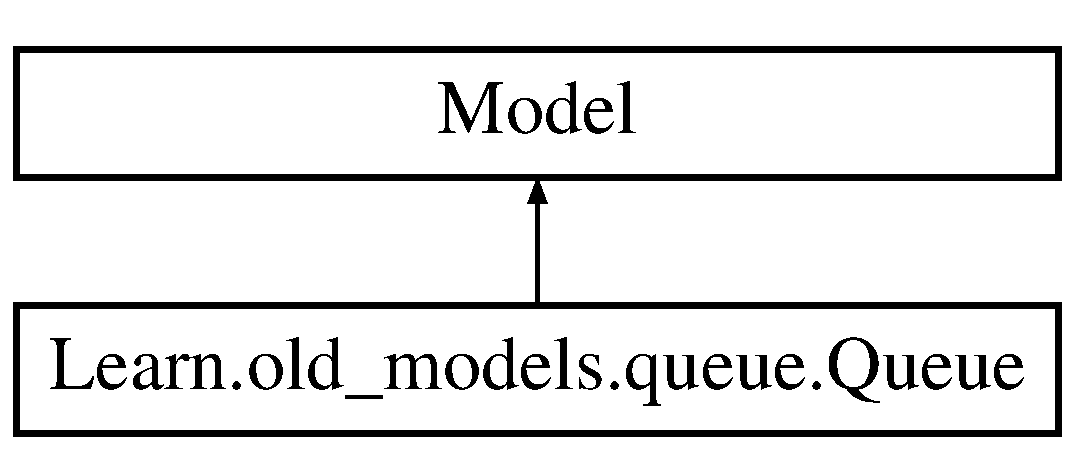
\includegraphics[height=2.000000cm]{class_learn_1_1old__models_1_1queue_1_1_queue}
\end{center}
\end{figure}
\subsection*{Classes}
\begin{DoxyCompactItemize}
\item 
class \hyperlink{class_learn_1_1old__models_1_1queue_1_1_queue_1_1_meta}{Meta}
\end{DoxyCompactItemize}
\subsection*{Static Public Attributes}
\begin{DoxyCompactItemize}
\item 
\hypertarget{class_learn_1_1old__models_1_1queue_1_1_queue_ab4de315be802ee31cd54062e7f73f081}{tuple {\bfseries uuid} models.\-Char\-Field(max\-\_\-length=36, primary\-\_\-key=True)}\label{class_learn_1_1old__models_1_1queue_1_1_queue_ab4de315be802ee31cd54062e7f73f081}

\item 
\hypertarget{class_learn_1_1old__models_1_1queue_1_1_queue_a4b12193e9283873068820743fb1963c5}{tuple {\bfseries title} models.\-Char\-Field(max\-\_\-length=100)}\label{class_learn_1_1old__models_1_1queue_1_1_queue_a4b12193e9283873068820743fb1963c5}

\end{DoxyCompactItemize}


The documentation for this class was generated from the following file\-:\begin{DoxyCompactItemize}
\item 
/\-Users/\-Charlie/\-Documents/\-Aptana Studio 3 Workspace/\-C\-M2301-\/9/\-C\-M2301/\-Learn/old\-\_\-models/queue.\-py\end{DoxyCompactItemize}

\hypertarget{classqueue_1_1_queue_item}{\section{queue.\-Queue\-Item Class Reference}
\label{classqueue_1_1_queue_item}\index{queue.\-Queue\-Item@{queue.\-Queue\-Item}}
}
Inheritance diagram for queue.\-Queue\-Item\-:\begin{figure}[H]
\begin{center}
\leavevmode
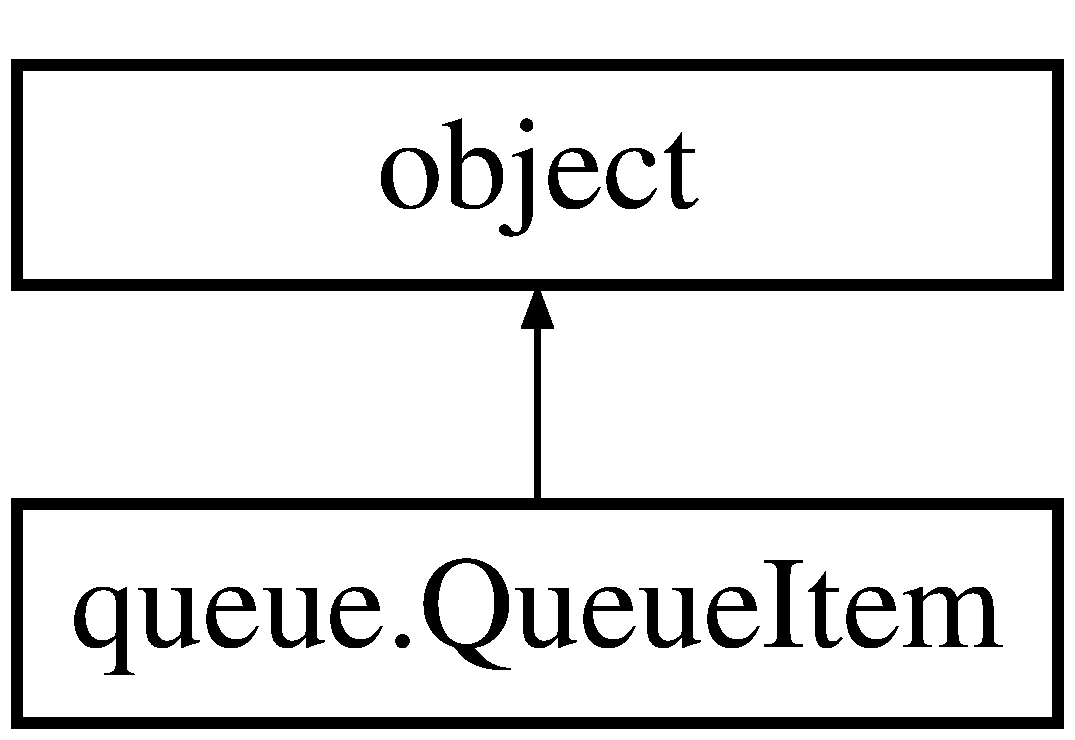
\includegraphics[height=2.000000cm]{classqueue_1_1_queue_item}
\end{center}
\end{figure}
\subsection*{Public Member Functions}
\begin{DoxyCompactItemize}
\item 
\hypertarget{classqueue_1_1_queue_item_ae0d58fab209ae5eed884fb99a0af8686}{def {\bfseries \-\_\-\-\_\-init\-\_\-\-\_\-}}\label{classqueue_1_1_queue_item_ae0d58fab209ae5eed884fb99a0af8686}

\item 
\hypertarget{classqueue_1_1_queue_item_a319a260d27889634770fa945b7b673a8}{def \hyperlink{classqueue_1_1_queue_item_a319a260d27889634770fa945b7b673a8}{save}}\label{classqueue_1_1_queue_item_a319a260d27889634770fa945b7b673a8}

\begin{DoxyCompactList}\small\item\em Saves the queue item back to the database. \end{DoxyCompactList}\end{DoxyCompactItemize}
\subsection*{Static Public Attributes}
\begin{DoxyCompactItemize}
\item 
\hypertarget{classqueue_1_1_queue_item_af790caa69632f7d36059c340ff572efe}{{\bfseries uuid} None}\label{classqueue_1_1_queue_item_af790caa69632f7d36059c340ff572efe}

\item 
\hypertarget{classqueue_1_1_queue_item_ad7f6afef5067cd89c2c44193e46171a0}{{\bfseries job\-\_\-type} None}\label{classqueue_1_1_queue_item_ad7f6afef5067cd89c2c44193e46171a0}

\item 
\hypertarget{classqueue_1_1_queue_item_aa8f8230cef6f9211acd084f9acb9ecb7}{{\bfseries submission\-\_\-time} None}\label{classqueue_1_1_queue_item_aa8f8230cef6f9211acd084f9acb9ecb7}

\item 
\hypertarget{classqueue_1_1_queue_item_a0eebd4a1885a8192f6a440109e8ae9e1}{{\bfseries waiting} False}\label{classqueue_1_1_queue_item_a0eebd4a1885a8192f6a440109e8ae9e1}

\item 
\hypertarget{classqueue_1_1_queue_item_a1d6ef7968231fead6f07a913d0031d2e}{float {\bfseries progress} 0.\-0}\label{classqueue_1_1_queue_item_a1d6ef7968231fead6f07a913d0031d2e}

\item 
\hypertarget{classqueue_1_1_queue_item_a8c232bf9d64d8b0095eab9faffc94daf}{{\bfseries completion\-\_\-time} None}\label{classqueue_1_1_queue_item_a8c232bf9d64d8b0095eab9faffc94daf}

\end{DoxyCompactItemize}


The documentation for this class was generated from the following file\-:\begin{DoxyCompactItemize}
\item 
/\-Users/\-Charlie/\-Documents/\-Aptana Studio 3 Workspace/\-C\-M2301-\/9/\-Server/queue.\-py\end{DoxyCompactItemize}

\hypertarget{classqueue_1_1_queue_manager}{\section{queue.\-Queue\-Manager Class Reference}
\label{classqueue_1_1_queue_manager}\index{queue.\-Queue\-Manager@{queue.\-Queue\-Manager}}
}
Inheritance diagram for queue.\-Queue\-Manager\-:\begin{figure}[H]
\begin{center}
\leavevmode
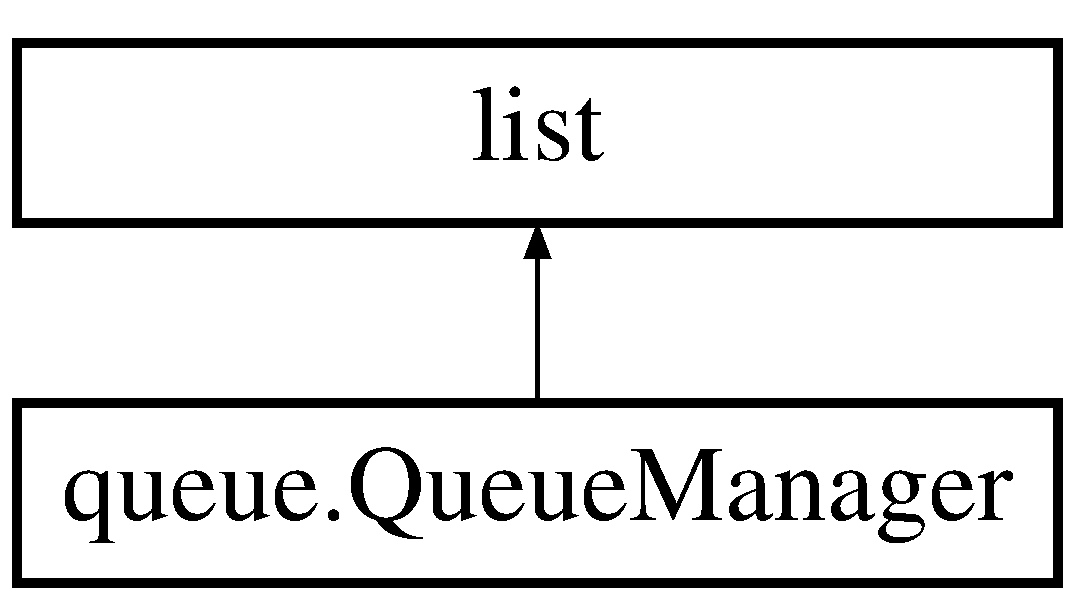
\includegraphics[height=2.000000cm]{classqueue_1_1_queue_manager}
\end{center}
\end{figure}
\subsection*{Public Member Functions}
\begin{DoxyCompactItemize}
\item 
\hypertarget{classqueue_1_1_queue_manager_ae77c301f551c82782848d0523ae1595c}{def {\bfseries \-\_\-\-\_\-init\-\_\-\-\_\-}}\label{classqueue_1_1_queue_manager_ae77c301f551c82782848d0523ae1595c}

\item 
\hypertarget{classqueue_1_1_queue_manager_a361e2ff2a1dbeb3491964a2a48af1981}{def \hyperlink{classqueue_1_1_queue_manager_a361e2ff2a1dbeb3491964a2a48af1981}{get\-\_\-pending\-\_\-queue}}\label{classqueue_1_1_queue_manager_a361e2ff2a1dbeb3491964a2a48af1981}

\begin{DoxyCompactList}\small\item\em Fetches all uncomplete queue items from db. \end{DoxyCompactList}\end{DoxyCompactItemize}


The documentation for this class was generated from the following file\-:\begin{DoxyCompactItemize}
\item 
/\-Users/\-Charlie/\-Documents/\-Aptana Studio 3 Workspace/\-C\-M2301-\/9/\-Server/queue.\-py\end{DoxyCompactItemize}

\hypertarget{class_learn_1_1models_1_1_result}{\section{Learn.\-models.\-Result Class Reference}
\label{class_learn_1_1models_1_1_result}\index{Learn.\-models.\-Result@{Learn.\-models.\-Result}}
}


The result class stores a reference to the answer selected for a single question in a test, belonging to a \hyperlink{class_learn_1_1models_1_1_test_instance}{Test\-Instance}.  


Inheritance diagram for Learn.\-models.\-Result\-:\begin{figure}[H]
\begin{center}
\leavevmode
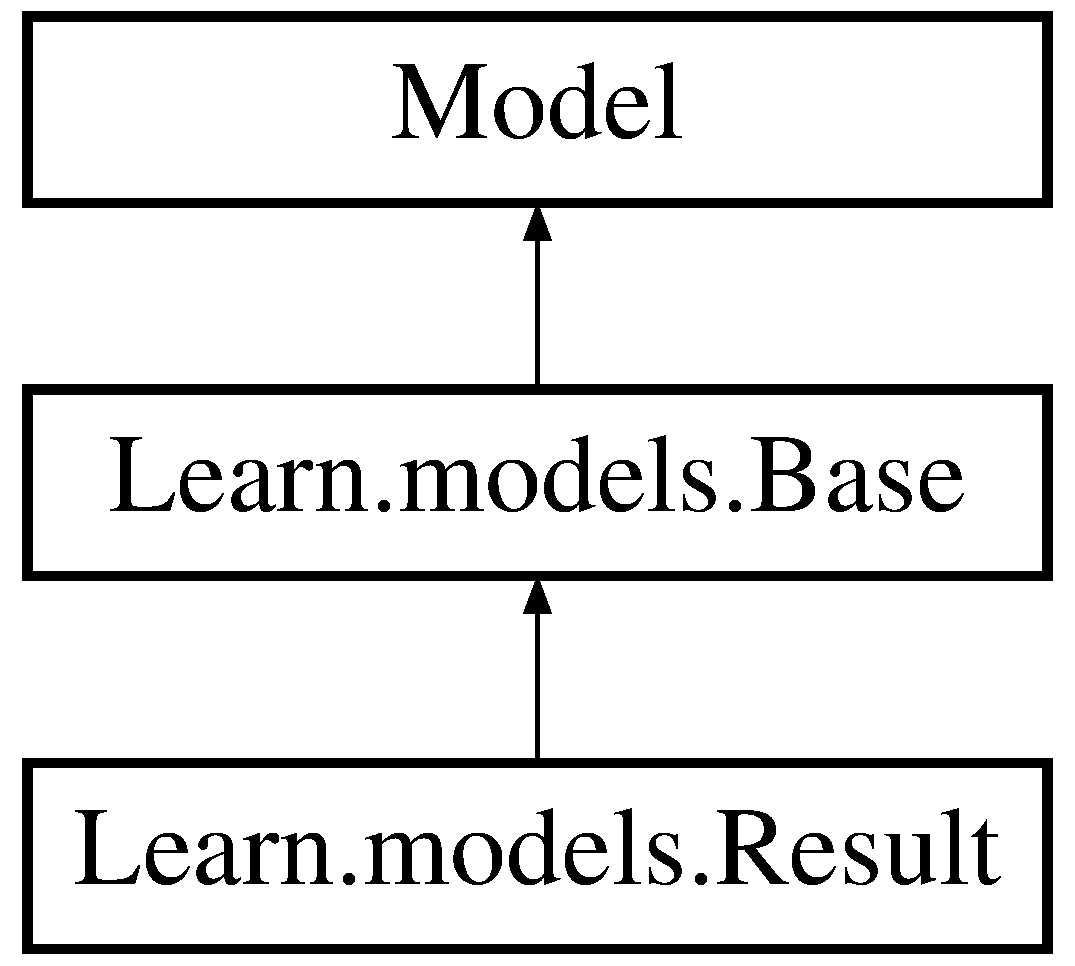
\includegraphics[height=3.000000cm]{class_learn_1_1models_1_1_result}
\end{center}
\end{figure}
\subsection*{Static Public Attributes}
\begin{DoxyCompactItemize}
\item 
\hypertarget{class_learn_1_1models_1_1_result_a94edab0375399fb6ed6d5987815589dc}{tuple {\bfseries test\-\_\-instance} models.\-Foreign\-Key(\hyperlink{class_learn_1_1models_1_1_test_instance}{Test\-Instance})}\label{class_learn_1_1models_1_1_result_a94edab0375399fb6ed6d5987815589dc}

\item 
\hypertarget{class_learn_1_1models_1_1_result_a22b220ee0d27909efb470049c3d642af}{tuple {\bfseries question} models.\-Foreign\-Key(\hyperlink{class_learn_1_1models_1_1_question}{Question})}\label{class_learn_1_1models_1_1_result_a22b220ee0d27909efb470049c3d642af}

\item 
\hypertarget{class_learn_1_1models_1_1_result_aab5cdf32ea6736df41d96f7eb33baca7}{tuple {\bfseries answer} models.\-Foreign\-Key(\hyperlink{class_learn_1_1models_1_1_answer}{Answer})}\label{class_learn_1_1models_1_1_result_aab5cdf32ea6736df41d96f7eb33baca7}

\end{DoxyCompactItemize}
\subsection*{Additional Inherited Members}


\subsection{Detailed Description}
The result class stores a reference to the answer selected for a single question in a test, belonging to a \hyperlink{class_learn_1_1models_1_1_test_instance}{Test\-Instance}. 

The documentation for this class was generated from the following file\-:\begin{DoxyCompactItemize}
\item 
/\-Users/\-Charlie/\-Documents/\-Aptana Studio 3 Workspace/\-C\-M2301-\/9/\-C\-M2301/\-Learn/models.\-py\end{DoxyCompactItemize}

\hypertarget{class_learn_1_1models_1_1_revision}{\section{Learn.\-models.\-Revision Class Reference}
\label{class_learn_1_1models_1_1_revision}\index{Learn.\-models.\-Revision@{Learn.\-models.\-Revision}}
}


A revision object represents a single file that belongs to an \hyperlink{class_learn_1_1models_1_1_attachment}{Attachment}.  


Inheritance diagram for Learn.\-models.\-Revision\-:\begin{figure}[H]
\begin{center}
\leavevmode
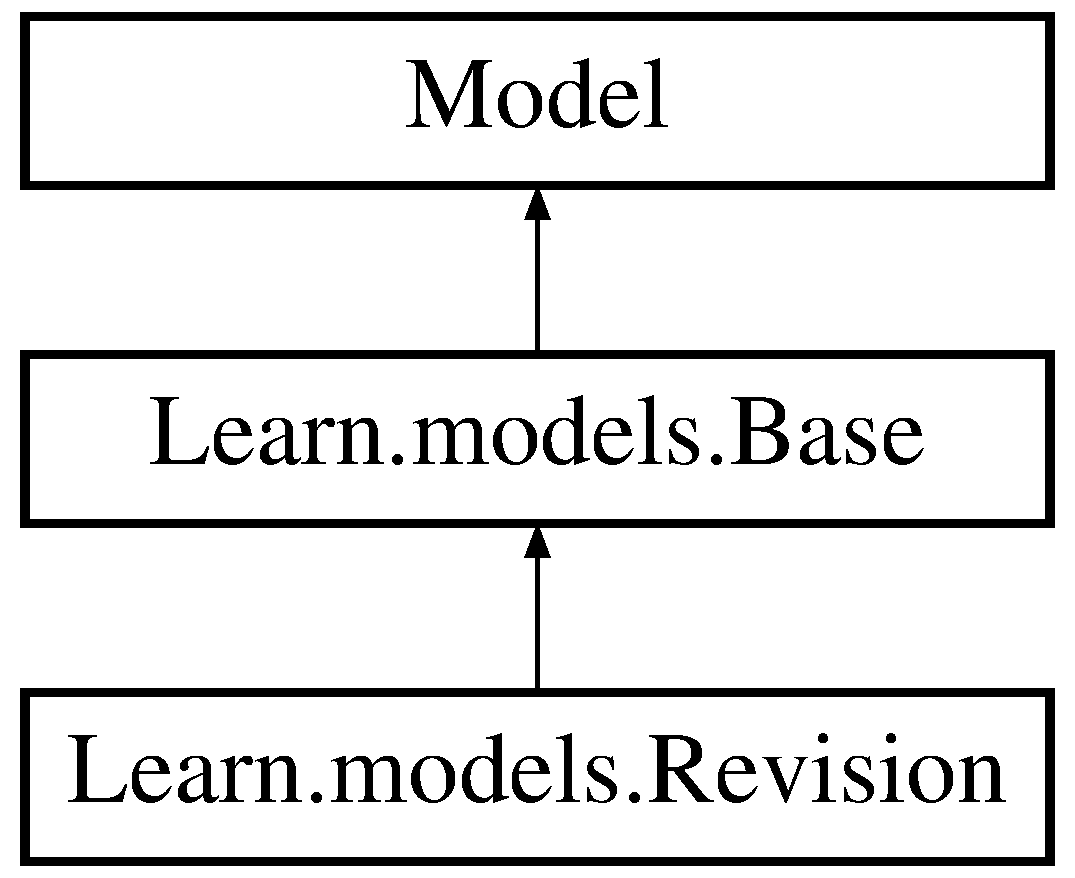
\includegraphics[height=3.000000cm]{class_learn_1_1models_1_1_revision}
\end{center}
\end{figure}
\subsection*{Public Member Functions}
\begin{DoxyCompactItemize}
\item 
def \hyperlink{class_learn_1_1models_1_1_revision_aba5613cb5880b9c860f2713d4528e80e}{get\-\_\-file}
\begin{DoxyCompactList}\small\item\em Returns the File object for the current \hyperlink{class_learn_1_1models_1_1_revision}{Revision}. \end{DoxyCompactList}\end{DoxyCompactItemize}
\subsection*{Static Public Attributes}
\begin{DoxyCompactItemize}
\item 
\hypertarget{class_learn_1_1models_1_1_revision_ab99a5799125da47290ffeca85fb4d290}{tuple \hyperlink{class_learn_1_1models_1_1_revision_ab99a5799125da47290ffeca85fb4d290}{time\-\_\-uploaded} models.\-Date\-Time\-Field(auto\-\_\-now\-\_\-add=True)}\label{class_learn_1_1models_1_1_revision_ab99a5799125da47290ffeca85fb4d290}

\begin{DoxyCompactList}\small\item\em The timestamp the document was uploaded/attached to the revision. \end{DoxyCompactList}\item 
tuple \hyperlink{class_learn_1_1models_1_1_revision_a1e0c1e0fafeb906c3ed10e882571f9e2}{attachment} models.\-Foreign\-Key(\hyperlink{class_learn_1_1models_1_1_attachment}{Attachment})
\begin{DoxyCompactList}\small\item\em The \hyperlink{class_learn_1_1models_1_1_attachment}{Attachment} object the \hyperlink{class_learn_1_1models_1_1_revision}{Revision} belongs to. \end{DoxyCompactList}\item 
\hypertarget{class_learn_1_1models_1_1_revision_ab6a44857b140b43e3dd0345a7bd94284}{tuple \hyperlink{class_learn_1_1models_1_1_revision_ab6a44857b140b43e3dd0345a7bd94284}{file} models.\-File\-Field(upload\-\_\-to='/')}\label{class_learn_1_1models_1_1_revision_ab6a44857b140b43e3dd0345a7bd94284}

\begin{DoxyCompactList}\small\item\em The File Object. \end{DoxyCompactList}\item 
\hypertarget{class_learn_1_1models_1_1_revision_a6bb6313e61fc4d6199b11c67ce6ea781}{tuple \hyperlink{class_learn_1_1models_1_1_revision_a6bb6313e61fc4d6199b11c67ce6ea781}{approved} models.\-Boolean\-Field()}\label{class_learn_1_1models_1_1_revision_a6bb6313e61fc4d6199b11c67ce6ea781}

\begin{DoxyCompactList}\small\item\em Whether or not the \hyperlink{class_learn_1_1models_1_1_revision}{Revision} has been approved. \end{DoxyCompactList}\item 
tuple \hyperlink{class_learn_1_1models_1_1_revision_aba129f90cca558a21d55c49935ee0c1a}{uploaded\-\_\-by} models.\-Foreign\-Key(\hyperlink{class_learn_1_1models_1_1_user}{User})
\begin{DoxyCompactList}\small\item\em The \hyperlink{class_learn_1_1models_1_1_user}{User} whom owns the \hyperlink{class_learn_1_1models_1_1_revision}{Revision} -\/ Usually the uploader. \end{DoxyCompactList}\item 
tuple \hyperlink{class_learn_1_1models_1_1_revision_ace081e49efb42548cc69b3f4dd13d0fb}{file\-\_\-size} models.\-Float\-Field()
\begin{DoxyCompactList}\small\item\em The file size of the \hyperlink{class_learn_1_1models_1_1_revision}{Revision} file. \end{DoxyCompactList}\end{DoxyCompactItemize}


\subsection{Detailed Description}
A revision object represents a single file that belongs to an \hyperlink{class_learn_1_1models_1_1_attachment}{Attachment}. 

This class facilitates \hyperlink{class_learn_1_1models_1_1_attachment}{Attachment} versioning 

\subsection{Member Function Documentation}
\hypertarget{class_learn_1_1models_1_1_revision_aba5613cb5880b9c860f2713d4528e80e}{\index{Learn\-::models\-::\-Revision@{Learn\-::models\-::\-Revision}!get\-\_\-file@{get\-\_\-file}}
\index{get\-\_\-file@{get\-\_\-file}!Learn::models::Revision@{Learn\-::models\-::\-Revision}}
\subsubsection[{get\-\_\-file}]{\setlength{\rightskip}{0pt plus 5cm}def Learn.\-models.\-Revision.\-get\-\_\-file (
\begin{DoxyParamCaption}
\item[{}]{self}
\end{DoxyParamCaption}
)}}\label{class_learn_1_1models_1_1_revision_aba5613cb5880b9c860f2713d4528e80e}


Returns the File object for the current \hyperlink{class_learn_1_1models_1_1_revision}{Revision}. 

\begin{DoxyReturn}{Returns}
File Returns the File handler for the \hyperlink{class_learn_1_1models_1_1_revision}{Revision} 
\end{DoxyReturn}


\subsection{Member Data Documentation}
\hypertarget{class_learn_1_1models_1_1_revision_a1e0c1e0fafeb906c3ed10e882571f9e2}{\index{Learn\-::models\-::\-Revision@{Learn\-::models\-::\-Revision}!attachment@{attachment}}
\index{attachment@{attachment}!Learn::models::Revision@{Learn\-::models\-::\-Revision}}
\subsubsection[{attachment}]{\setlength{\rightskip}{0pt plus 5cm}tuple Learn.\-models.\-Revision.\-attachment models.\-Foreign\-Key({\bf Attachment})\hspace{0.3cm}{\ttfamily [static]}}}\label{class_learn_1_1models_1_1_revision_a1e0c1e0fafeb906c3ed10e882571f9e2}


The \hyperlink{class_learn_1_1models_1_1_attachment}{Attachment} object the \hyperlink{class_learn_1_1models_1_1_revision}{Revision} belongs to. 

\hypertarget{class_learn_1_1models_1_1_revision_ace081e49efb42548cc69b3f4dd13d0fb}{\index{Learn\-::models\-::\-Revision@{Learn\-::models\-::\-Revision}!file\-\_\-size@{file\-\_\-size}}
\index{file\-\_\-size@{file\-\_\-size}!Learn::models::Revision@{Learn\-::models\-::\-Revision}}
\subsubsection[{file\-\_\-size}]{\setlength{\rightskip}{0pt plus 5cm}tuple Learn.\-models.\-Revision.\-file\-\_\-size models.\-Float\-Field()\hspace{0.3cm}{\ttfamily [static]}}}\label{class_learn_1_1models_1_1_revision_ace081e49efb42548cc69b3f4dd13d0fb}


The file size of the \hyperlink{class_learn_1_1models_1_1_revision}{Revision} file. 

\hypertarget{class_learn_1_1models_1_1_revision_aba129f90cca558a21d55c49935ee0c1a}{\index{Learn\-::models\-::\-Revision@{Learn\-::models\-::\-Revision}!uploaded\-\_\-by@{uploaded\-\_\-by}}
\index{uploaded\-\_\-by@{uploaded\-\_\-by}!Learn::models::Revision@{Learn\-::models\-::\-Revision}}
\subsubsection[{uploaded\-\_\-by}]{\setlength{\rightskip}{0pt plus 5cm}tuple Learn.\-models.\-Revision.\-uploaded\-\_\-by models.\-Foreign\-Key({\bf User})\hspace{0.3cm}{\ttfamily [static]}}}\label{class_learn_1_1models_1_1_revision_aba129f90cca558a21d55c49935ee0c1a}


The \hyperlink{class_learn_1_1models_1_1_user}{User} whom owns the \hyperlink{class_learn_1_1models_1_1_revision}{Revision} -\/ Usually the uploader. 



The documentation for this class was generated from the following file\-:\begin{DoxyCompactItemize}
\item 
/\-Users/\-Charlie/\-Documents/\-Aptana Studio 3 Workspace/\-C\-M2301-\/9/\-C\-M2301/\-Learn/models.\-py\end{DoxyCompactItemize}

\hypertarget{classserver__load_1_1_server_load}{\section{server\-\_\-load.\-Server\-Load Class Reference}
\label{classserver__load_1_1_server_load}\index{server\-\_\-load.\-Server\-Load@{server\-\_\-load.\-Server\-Load}}
}
Inheritance diagram for server\-\_\-load.\-Server\-Load\-:\begin{figure}[H]
\begin{center}
\leavevmode
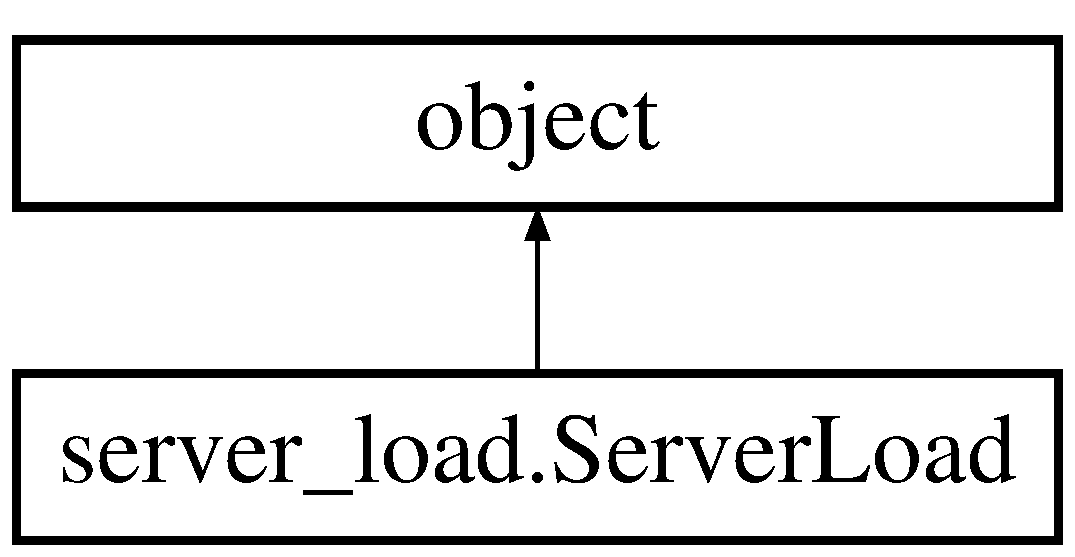
\includegraphics[height=2.000000cm]{classserver__load_1_1_server_load}
\end{center}
\end{figure}
\subsection*{Public Member Functions}
\begin{DoxyCompactItemize}
\item 
\hypertarget{classserver__load_1_1_server_load_aafc2d53d586363c7fe6a079137881710}{def {\bfseries \-\_\-\-\_\-init\-\_\-\-\_\-}}\label{classserver__load_1_1_server_load_aafc2d53d586363c7fe6a079137881710}

\item 
\hypertarget{classserver__load_1_1_server_load_acd4ebfbb9683857645e04954fe08134c}{def \hyperlink{classserver__load_1_1_server_load_acd4ebfbb9683857645e04954fe08134c}{persist\-\_\-load}}\label{classserver__load_1_1_server_load_acd4ebfbb9683857645e04954fe08134c}

\begin{DoxyCompactList}\small\item\em Saves the current server load to the database. \end{DoxyCompactList}\item 
\hypertarget{classserver__load_1_1_server_load_a75ed333bf4bb28ecc70a4f7f1f8ee335}{def \hyperlink{classserver__load_1_1_server_load_a75ed333bf4bb28ecc70a4f7f1f8ee335}{update\-\_\-load}}\label{classserver__load_1_1_server_load_a75ed333bf4bb28ecc70a4f7f1f8ee335}

\begin{DoxyCompactList}\small\item\em Updates the historical load list, capped to 60 and is a blocking method. \end{DoxyCompactList}\item 
\hypertarget{classserver__load_1_1_server_load_ab0c0ac1a48191a7cb144cec07127b0a1}{def \hyperlink{classserver__load_1_1_server_load_ab0c0ac1a48191a7cb144cec07127b0a1}{calculate\-\_\-load}}\label{classserver__load_1_1_server_load_ab0c0ac1a48191a7cb144cec07127b0a1}

\begin{DoxyCompactList}\small\item\em Returns the actual useful load! \end{DoxyCompactList}\item 
\hypertarget{classserver__load_1_1_server_load_a455c7fce4e73b4aec74cf6ae2fe265a2}{def \hyperlink{classserver__load_1_1_server_load_a455c7fce4e73b4aec74cf6ae2fe265a2}{start\-\_\-updating}}\label{classserver__load_1_1_server_load_a455c7fce4e73b4aec74cf6ae2fe265a2}

\begin{DoxyCompactList}\small\item\em Stards the object logging load. \end{DoxyCompactList}\item 
\hypertarget{classserver__load_1_1_server_load_a2ed75baaef3506087099b41fac09607f}{def \hyperlink{classserver__load_1_1_server_load_a2ed75baaef3506087099b41fac09607f}{stop\-\_\-updating}}\label{classserver__load_1_1_server_load_a2ed75baaef3506087099b41fac09607f}

\begin{DoxyCompactList}\small\item\em Stops the object logging load. \end{DoxyCompactList}\end{DoxyCompactItemize}
\subsection*{Public Attributes}
\begin{DoxyCompactItemize}
\item 
\hypertarget{classserver__load_1_1_server_load_a8103c4ebb72f0aae7f449763b0d0bb42}{{\bfseries last\-\_\-update}}\label{classserver__load_1_1_server_load_a8103c4ebb72f0aae7f449763b0d0bb42}

\end{DoxyCompactItemize}
\subsection*{Static Public Attributes}
\begin{DoxyCompactItemize}
\item 
\hypertarget{classserver__load_1_1_server_load_a93a602d7751152367edeaefad7983f4b}{list {\bfseries server\-\_\-load} \mbox{[}$\,$\mbox{]}}\label{classserver__load_1_1_server_load_a93a602d7751152367edeaefad7983f4b}

\item 
\hypertarget{classserver__load_1_1_server_load_ac1331cbdfbd9ba2f409cc32115942503}{list {\bfseries cpu\-\_\-usage} \mbox{[}$\,$\mbox{]}}\label{classserver__load_1_1_server_load_ac1331cbdfbd9ba2f409cc32115942503}

\item 
\hypertarget{classserver__load_1_1_server_load_a51fc6e20e8b3453951e593dc440b842a}{float {\bfseries mem\-\_\-usage} 0.\-0}\label{classserver__load_1_1_server_load_a51fc6e20e8b3453951e593dc440b842a}

\item 
\hypertarget{classserver__load_1_1_server_load_a98844d6088ecfc744e862a56070567ad}{float {\bfseries last\-\_\-update} 0.\-0}\label{classserver__load_1_1_server_load_a98844d6088ecfc744e862a56070567ad}

\item 
\hypertarget{classserver__load_1_1_server_load_a13b008930cefb3207abfc8e296d84c13}{{\bfseries updating} False}\label{classserver__load_1_1_server_load_a13b008930cefb3207abfc8e296d84c13}

\end{DoxyCompactItemize}


The documentation for this class was generated from the following file\-:\begin{DoxyCompactItemize}
\item 
/\-Users/\-Charlie/\-Documents/\-Aptana Studio 3 Workspace/\-C\-M2301-\/9/\-Server/server\-\_\-load.\-py\end{DoxyCompactItemize}

\hypertarget{class_learn_1_1tests_1_1_simple_test}{\section{Learn.\-tests.\-Simple\-Test Class Reference}
\label{class_learn_1_1tests_1_1_simple_test}\index{Learn.\-tests.\-Simple\-Test@{Learn.\-tests.\-Simple\-Test}}
}
Inheritance diagram for Learn.\-tests.\-Simple\-Test\-:\begin{figure}[H]
\begin{center}
\leavevmode
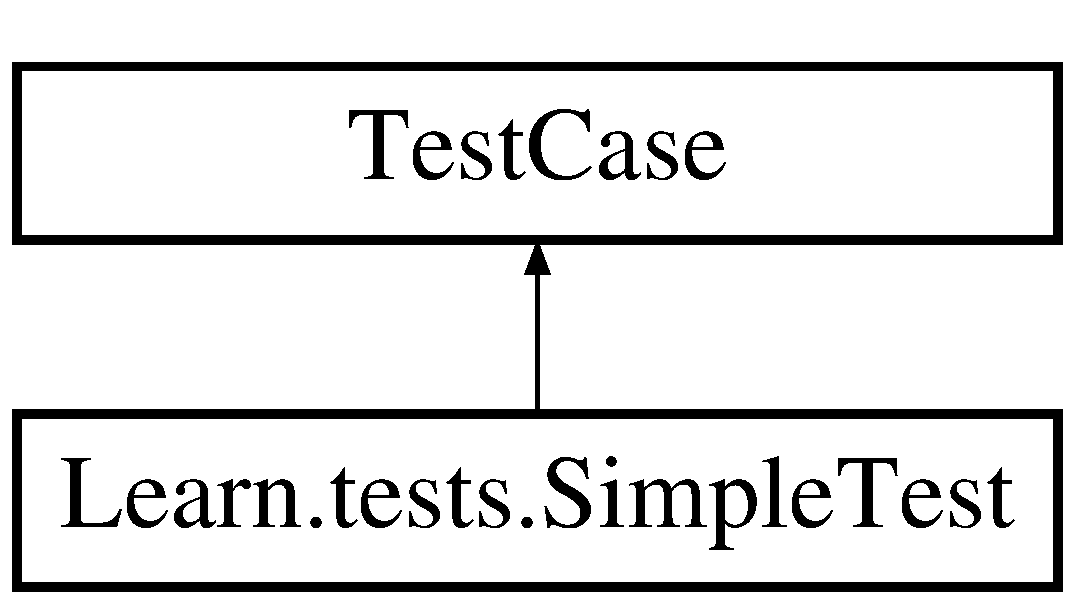
\includegraphics[height=2.000000cm]{class_learn_1_1tests_1_1_simple_test}
\end{center}
\end{figure}
\subsection*{Public Member Functions}
\begin{DoxyCompactItemize}
\item 
\hypertarget{class_learn_1_1tests_1_1_simple_test_a89c70e1c14de8d213e92746d1e0ece06}{def \hyperlink{class_learn_1_1tests_1_1_simple_test_a89c70e1c14de8d213e92746d1e0ece06}{test\-\_\-basic\-\_\-addition}}\label{class_learn_1_1tests_1_1_simple_test_a89c70e1c14de8d213e92746d1e0ece06}

\begin{DoxyCompactList}\small\item\em Tests that 1 + 1 always equals 2. \end{DoxyCompactList}\end{DoxyCompactItemize}


The documentation for this class was generated from the following file\-:\begin{DoxyCompactItemize}
\item 
/\-Users/\-Charlie/\-Documents/\-Aptana Studio 3 Workspace/\-C\-M2301-\/9/\-C\-M2301/\-Learn/tests.\-py\end{DoxyCompactItemize}

\hypertarget{class_learn_1_1old__models_1_1student_1_1_student}{\section{Learn.\-old\-\_\-models.\-student.\-Student Class Reference}
\label{class_learn_1_1old__models_1_1student_1_1_student}\index{Learn.\-old\-\_\-models.\-student.\-Student@{Learn.\-old\-\_\-models.\-student.\-Student}}
}
Inheritance diagram for Learn.\-old\-\_\-models.\-student.\-Student\-:\begin{figure}[H]
\begin{center}
\leavevmode
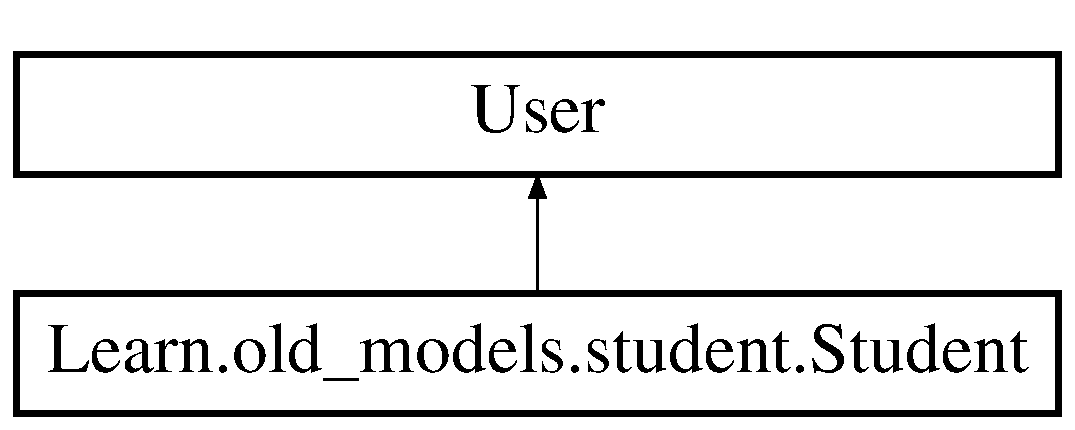
\includegraphics[height=2.000000cm]{class_learn_1_1old__models_1_1student_1_1_student}
\end{center}
\end{figure}
\subsection*{Classes}
\begin{DoxyCompactItemize}
\item 
class \hyperlink{class_learn_1_1old__models_1_1student_1_1_student_1_1_meta}{Meta}
\end{DoxyCompactItemize}
\subsection*{Static Public Attributes}
\begin{DoxyCompactItemize}
\item 
\hypertarget{class_learn_1_1old__models_1_1student_1_1_student_a1011bce73e302f1ec27b71ac0bf19507}{tuple {\bfseries student\-\_\-number} models.\-Char\-Field(max\-\_\-length=50)}\label{class_learn_1_1old__models_1_1student_1_1_student_a1011bce73e302f1ec27b71ac0bf19507}

\item 
\hypertarget{class_learn_1_1old__models_1_1student_1_1_student_a6685bee108a5a1d42f09ba5c4f6e32be}{tuple {\bfseries course\-\_\-enrolled} models.\-Char\-Field(max\-\_\-length=50)}\label{class_learn_1_1old__models_1_1student_1_1_student_a6685bee108a5a1d42f09ba5c4f6e32be}

\end{DoxyCompactItemize}


The documentation for this class was generated from the following file\-:\begin{DoxyCompactItemize}
\item 
/\-Users/\-Charlie/\-Documents/\-Aptana Studio 3 Workspace/\-C\-M2301-\/9/\-C\-M2301/\-Learn/old\-\_\-models/student.\-py\end{DoxyCompactItemize}

\hypertarget{class_learn_1_1models_1_1_test}{\section{Learn.\-models.\-Test Class Reference}
\label{class_learn_1_1models_1_1_test}\index{Learn.\-models.\-Test@{Learn.\-models.\-Test}}
}


An instance of the test class will contain details of the \hyperlink{class_learn_1_1models_1_1_test}{Test} with the lecture it belongs to.  


Inheritance diagram for Learn.\-models.\-Test\-:\begin{figure}[H]
\begin{center}
\leavevmode
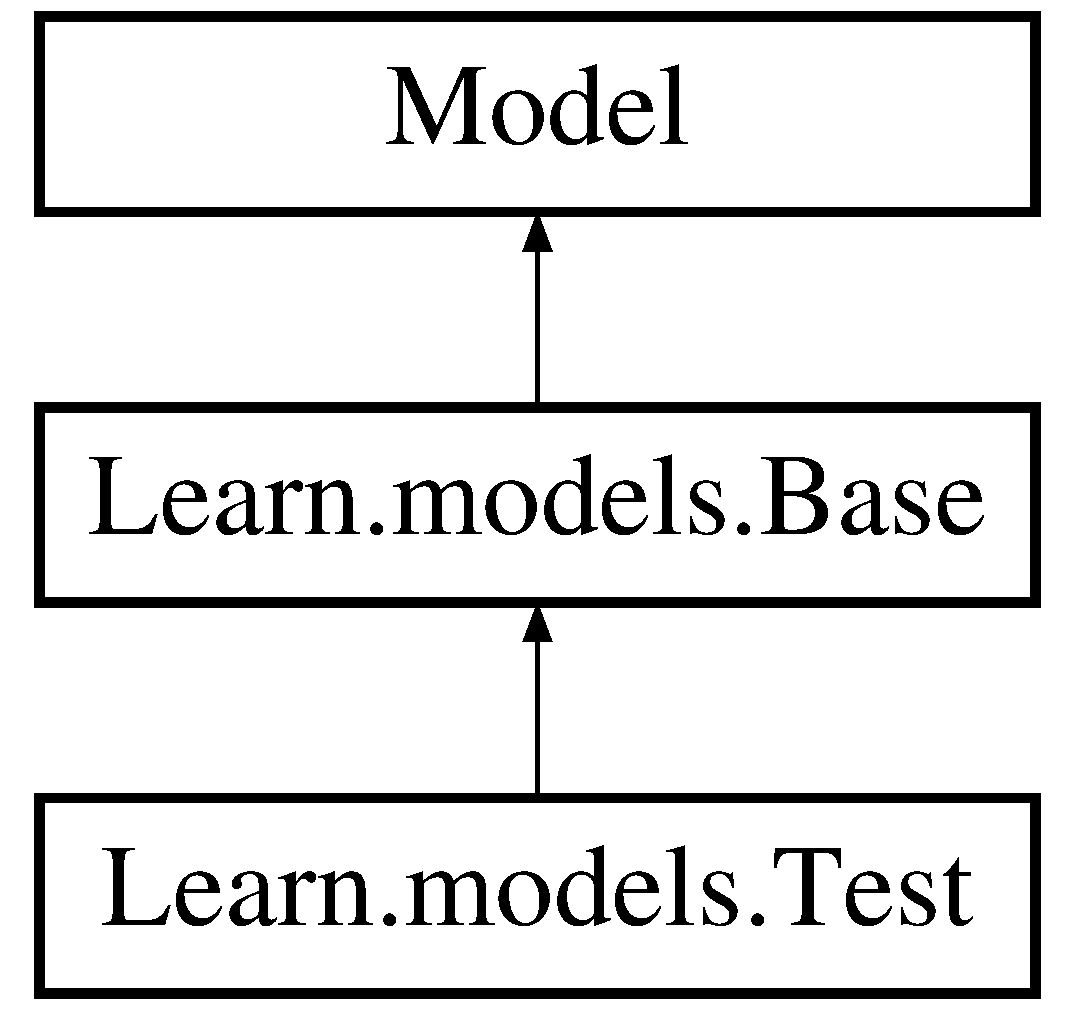
\includegraphics[height=3.000000cm]{class_learn_1_1models_1_1_test}
\end{center}
\end{figure}
\subsection*{Public Member Functions}
\begin{DoxyCompactItemize}
\item 
\hypertarget{class_learn_1_1models_1_1_test_a020a2bfa27be99f131c0c9491aff53f8}{def \hyperlink{class_learn_1_1models_1_1_test_a020a2bfa27be99f131c0c9491aff53f8}{get\-\_\-random\-\_\-questions}}\label{class_learn_1_1models_1_1_test_a020a2bfa27be99f131c0c9491aff53f8}

\begin{DoxyCompactList}\small\item\em Returns a List of random questions taken from the property Question\-List with the length of question\-Count, if question\-Count is larger than the length of Question\-List a Exception will be thrown. \end{DoxyCompactList}\end{DoxyCompactItemize}
\subsection*{Static Public Attributes}
\begin{DoxyCompactItemize}
\item 
\hypertarget{class_learn_1_1models_1_1_test_afa6b8269025be4e8a17d3d1259eec53b}{tuple {\bfseries title} models.\-Char\-Field(max\-\_\-length=250)}\label{class_learn_1_1models_1_1_test_afa6b8269025be4e8a17d3d1259eec53b}

\item 
\hypertarget{class_learn_1_1models_1_1_test_a1e99f210ccd11bf5b2dd55cab16d4384}{tuple {\bfseries description} models.\-Text\-Field()}\label{class_learn_1_1models_1_1_test_a1e99f210ccd11bf5b2dd55cab16d4384}

\item 
\hypertarget{class_learn_1_1models_1_1_test_a029d8b12971e04f78665d088b6a02961}{tuple {\bfseries question\-\_\-count} models.\-Integer\-Field()}\label{class_learn_1_1models_1_1_test_a029d8b12971e04f78665d088b6a02961}

\item 
\hypertarget{class_learn_1_1models_1_1_test_abac626d90f0bab225110dfd4c955e3d9}{tuple {\bfseries questions} models.\-Many\-To\-Many\-Field(\hyperlink{class_learn_1_1models_1_1_question}{Question})}\label{class_learn_1_1models_1_1_test_abac626d90f0bab225110dfd4c955e3d9}

\item 
\hypertarget{class_learn_1_1models_1_1_test_ab2cef470549f3fb48d3399faf4e8f446}{tuple {\bfseries lecture} models.\-Many\-To\-Many\-Field(\hyperlink{class_learn_1_1models_1_1_lecture}{Lecture})}\label{class_learn_1_1models_1_1_test_ab2cef470549f3fb48d3399faf4e8f446}

\end{DoxyCompactItemize}


\subsection{Detailed Description}
An instance of the test class will contain details of the \hyperlink{class_learn_1_1models_1_1_test}{Test} with the lecture it belongs to. 

As well as the full set of questions that could be asked. 

The documentation for this class was generated from the following file\-:\begin{DoxyCompactItemize}
\item 
/\-Users/\-Charlie/\-Documents/\-Aptana Studio 3 Workspace/\-C\-M2301-\/9/\-C\-M2301/\-Learn/models.\-py\end{DoxyCompactItemize}

\hypertarget{class_learn_1_1models_1_1_test_instance}{\section{Learn.\-models.\-Test\-Instance Class Reference}
\label{class_learn_1_1models_1_1_test_instance}\index{Learn.\-models.\-Test\-Instance@{Learn.\-models.\-Test\-Instance}}
}


A \hyperlink{class_learn_1_1models_1_1_test_instance}{Test\-Instance} object contains a reference to related \hyperlink{class_learn_1_1models_1_1_test}{Test}, the student completing it and the time it was completed.  


Inheritance diagram for Learn.\-models.\-Test\-Instance\-:\begin{figure}[H]
\begin{center}
\leavevmode
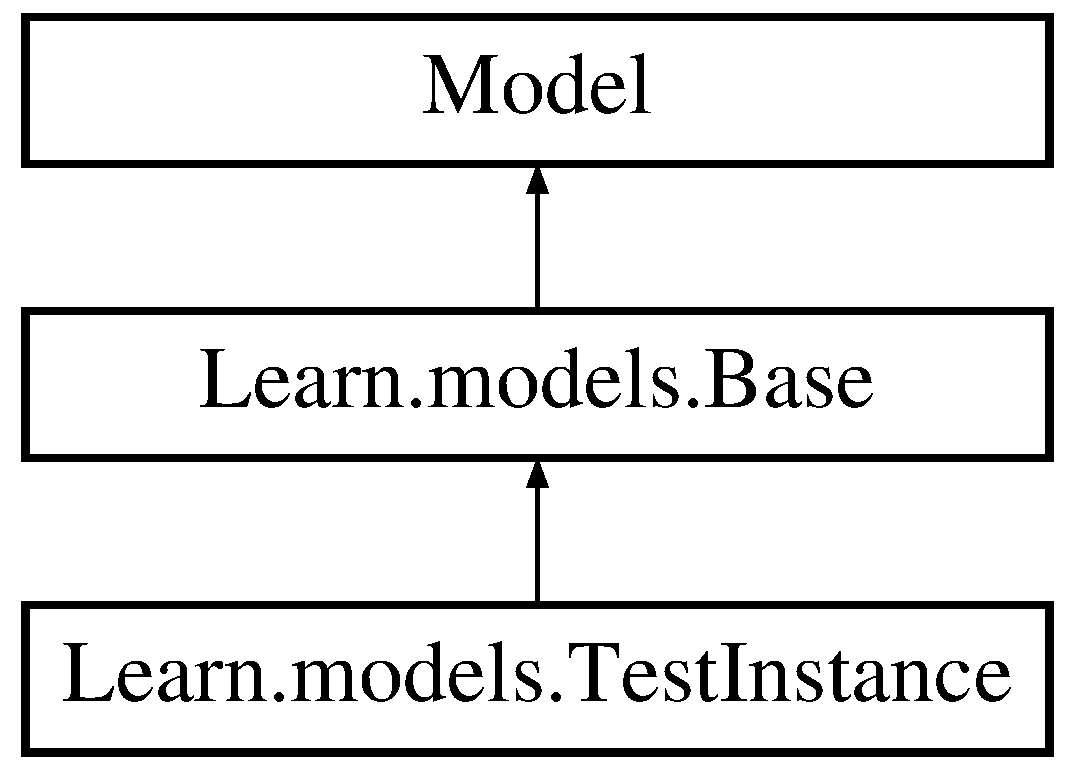
\includegraphics[height=3.000000cm]{class_learn_1_1models_1_1_test_instance}
\end{center}
\end{figure}
\subsection*{Public Member Functions}
\begin{DoxyCompactItemize}
\item 
\hypertarget{class_learn_1_1models_1_1_test_instance_ac5718c6c40673cfe7b1e6bdbc277c1d1}{def \hyperlink{class_learn_1_1models_1_1_test_instance_ac5718c6c40673cfe7b1e6bdbc277c1d1}{calc\-\_\-result}}\label{class_learn_1_1models_1_1_test_instance_ac5718c6c40673cfe7b1e6bdbc277c1d1}

\begin{DoxyCompactList}\small\item\em Returns the percentage of answers correct in the \hyperlink{class_learn_1_1models_1_1_test_instance}{Test\-Instance} as a float. \end{DoxyCompactList}\end{DoxyCompactItemize}
\subsection*{Static Public Attributes}
\begin{DoxyCompactItemize}
\item 
\hypertarget{class_learn_1_1models_1_1_test_instance_aba775978ffaff379df4ce0efe21c733f}{tuple {\bfseries student} models.\-Foreign\-Key(\hyperlink{class_learn_1_1models_1_1_user}{User})}\label{class_learn_1_1models_1_1_test_instance_aba775978ffaff379df4ce0efe21c733f}

\item 
\hypertarget{class_learn_1_1models_1_1_test_instance_a85d5a67bc7a423519d5ecd8b8040e2e9}{tuple {\bfseries test} models.\-Foreign\-Key(\hyperlink{class_learn_1_1models_1_1_test}{Test})}\label{class_learn_1_1models_1_1_test_instance_a85d5a67bc7a423519d5ecd8b8040e2e9}

\item 
\hypertarget{class_learn_1_1models_1_1_test_instance_a5c6218cd0a6245c7ea3e55c3671c91e9}{tuple {\bfseries time\-\_\-completed} models.\-Date\-Time\-Field()}\label{class_learn_1_1models_1_1_test_instance_a5c6218cd0a6245c7ea3e55c3671c91e9}

\end{DoxyCompactItemize}


\subsection{Detailed Description}
A \hyperlink{class_learn_1_1models_1_1_test_instance}{Test\-Instance} object contains a reference to related \hyperlink{class_learn_1_1models_1_1_test}{Test}, the student completing it and the time it was completed. 

The documentation for this class was generated from the following file\-:\begin{DoxyCompactItemize}
\item 
/\-Users/\-Charlie/\-Documents/\-Aptana Studio 3 Workspace/\-C\-M2301-\/9/\-C\-M2301/\-Learn/models.\-py\end{DoxyCompactItemize}

\hypertarget{class_learn_1_1models_1_1_user}{\section{Learn.\-models.\-User Class Reference}
\label{class_learn_1_1models_1_1_user}\index{Learn.\-models.\-User@{Learn.\-models.\-User}}
}


Represents a user of the system.  


Inheritance diagram for Learn.\-models.\-User\-:\begin{figure}[H]
\begin{center}
\leavevmode
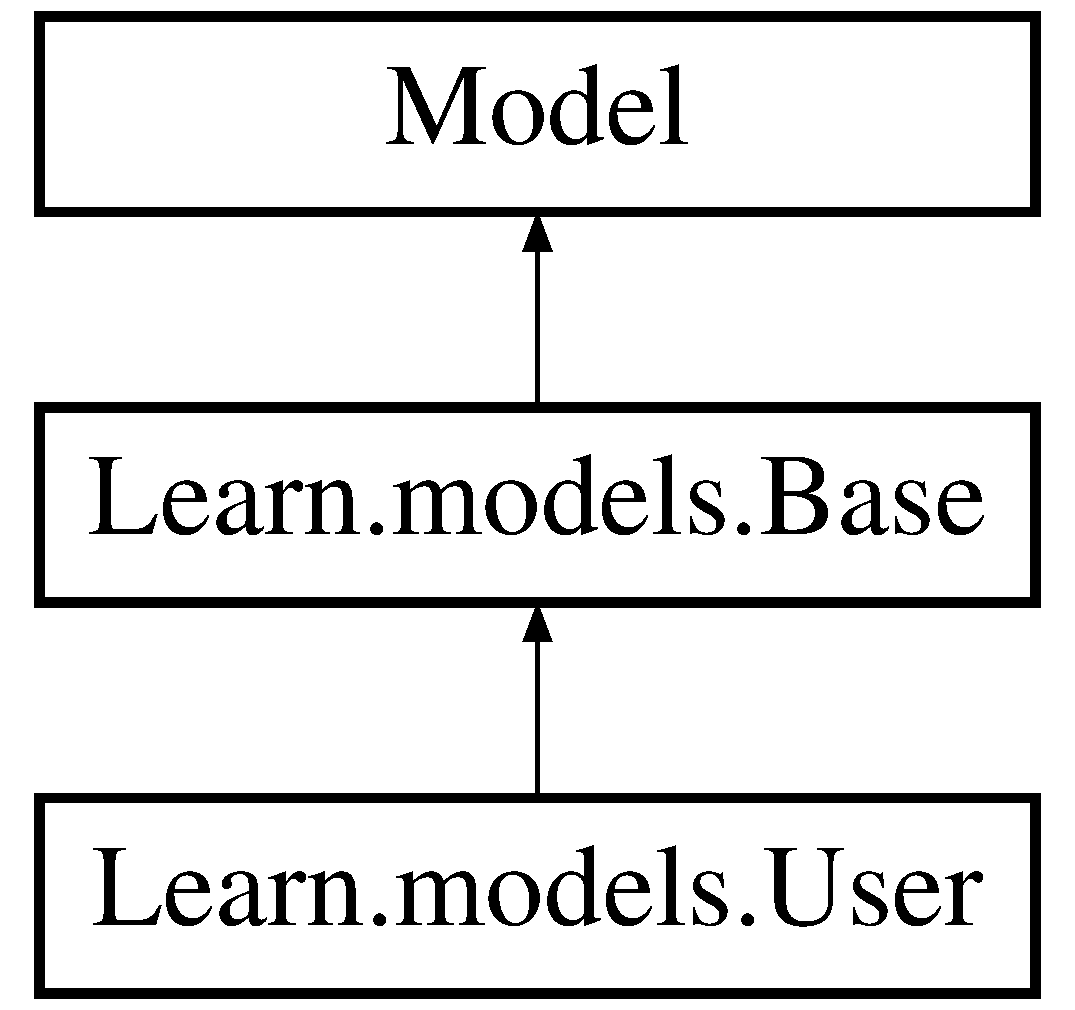
\includegraphics[height=3.000000cm]{class_learn_1_1models_1_1_user}
\end{center}
\end{figure}
\subsection*{Public Member Functions}
\begin{DoxyCompactItemize}
\item 
def \hyperlink{class_learn_1_1models_1_1_user_aefbdebc82f11edfa6de46493565b3bbc}{add\-\_\-user\-\_\-field}
\begin{DoxyCompactList}\small\item\em Adds a \hyperlink{class_learn_1_1models_1_1_user_field}{User\-Field} object to the \hyperlink{class_learn_1_1models_1_1_user}{User}. \end{DoxyCompactList}\end{DoxyCompactItemize}
\subsection*{Static Public Attributes}
\begin{DoxyCompactItemize}
\item 
\hypertarget{class_learn_1_1models_1_1_user_a90bee78e749e518923cbb4934582401a}{tuple \hyperlink{class_learn_1_1models_1_1_user_a90bee78e749e518923cbb4934582401a}{forename} models.\-Char\-Field(max\-\_\-length=50)}\label{class_learn_1_1models_1_1_user_a90bee78e749e518923cbb4934582401a}

\begin{DoxyCompactList}\small\item\em Forename of the \hyperlink{class_learn_1_1models_1_1_user}{User}. \end{DoxyCompactList}\item 
\hypertarget{class_learn_1_1models_1_1_user_a2e5e150422fc3c1e31af7df2c0cfefb9}{tuple \hyperlink{class_learn_1_1models_1_1_user_a2e5e150422fc3c1e31af7df2c0cfefb9}{surname} models.\-Char\-Field(max\-\_\-length=50)}\label{class_learn_1_1models_1_1_user_a2e5e150422fc3c1e31af7df2c0cfefb9}

\begin{DoxyCompactList}\small\item\em Surname of the \hyperlink{class_learn_1_1models_1_1_user}{User}. \end{DoxyCompactList}\item 
\hypertarget{class_learn_1_1models_1_1_user_a042ac88deb5e3d1fb6022e318eae34b1}{tuple \hyperlink{class_learn_1_1models_1_1_user_a042ac88deb5e3d1fb6022e318eae34b1}{username} models.\-Char\-Field(max\-\_\-length=25)}\label{class_learn_1_1models_1_1_user_a042ac88deb5e3d1fb6022e318eae34b1}

\begin{DoxyCompactList}\small\item\em Username or alias for the \hyperlink{class_learn_1_1models_1_1_user}{User} object. \end{DoxyCompactList}\item 
\hypertarget{class_learn_1_1models_1_1_user_a7be9250587aecff1dc9b276b0fa7aa94}{tuple \hyperlink{class_learn_1_1models_1_1_user_a7be9250587aecff1dc9b276b0fa7aa94}{email} models.\-Email\-Field(max\-\_\-length=75)}\label{class_learn_1_1models_1_1_user_a7be9250587aecff1dc9b276b0fa7aa94}

\begin{DoxyCompactList}\small\item\em Email address registered with the \hyperlink{class_learn_1_1models_1_1_user}{User}. \end{DoxyCompactList}\item 
\hypertarget{class_learn_1_1models_1_1_user_ac5a80def84659153520d3ee4997b6823}{tuple \hyperlink{class_learn_1_1models_1_1_user_ac5a80def84659153520d3ee4997b6823}{phone} models.\-Char\-Field(max\-\_\-length=20)}\label{class_learn_1_1models_1_1_user_ac5a80def84659153520d3ee4997b6823}

\begin{DoxyCompactList}\small\item\em Phone number for the \hyperlink{class_learn_1_1models_1_1_user}{User}. \end{DoxyCompactList}\end{DoxyCompactItemize}


\subsection{Detailed Description}
Represents a user of the system. 

A \hyperlink{class_learn_1_1models_1_1_user}{User} contains attributes that are common for any user of the system. Other attributes can be linked with a user using the \hyperlink{class_learn_1_1models_1_1_user_field}{User\-Field} class 

\subsection{Member Function Documentation}
\hypertarget{class_learn_1_1models_1_1_user_aefbdebc82f11edfa6de46493565b3bbc}{\index{Learn\-::models\-::\-User@{Learn\-::models\-::\-User}!add\-\_\-user\-\_\-field@{add\-\_\-user\-\_\-field}}
\index{add\-\_\-user\-\_\-field@{add\-\_\-user\-\_\-field}!Learn::models::User@{Learn\-::models\-::\-User}}
\subsubsection[{add\-\_\-user\-\_\-field}]{\setlength{\rightskip}{0pt plus 5cm}def Learn.\-models.\-User.\-add\-\_\-user\-\_\-field (
\begin{DoxyParamCaption}
\item[{}]{self, }
\item[{}]{User\-Field}
\end{DoxyParamCaption}
)}}\label{class_learn_1_1models_1_1_user_aefbdebc82f11edfa6de46493565b3bbc}


Adds a \hyperlink{class_learn_1_1models_1_1_user_field}{User\-Field} object to the \hyperlink{class_learn_1_1models_1_1_user}{User}. 


\begin{DoxyParams}{Parameters}
{\em \hyperlink{class_learn_1_1models_1_1_user_field}{User\-Field}} & The \hyperlink{class_learn_1_1models_1_1_user_field}{User\-Field} object to set as belonging to the user. \\
\hline
\end{DoxyParams}
\begin{DoxyReturn}{Returns}
\hyperlink{class_learn_1_1models_1_1_user_field}{User\-Field} Returns the \hyperlink{class_learn_1_1models_1_1_user_field}{User\-Field} added. 
\end{DoxyReturn}

\begin{DoxyExceptions}{Exceptions}
{\em User\-Data\-Exception} & \\
\hline
\end{DoxyExceptions}


The documentation for this class was generated from the following file\-:\begin{DoxyCompactItemize}
\item 
/\-Users/\-Charlie/\-Documents/\-Aptana Studio 3 Workspace/\-C\-M2301-\/9/\-C\-M2301/\-Learn/models.\-py\end{DoxyCompactItemize}

\hypertarget{class_learn_1_1old__models_1_1user_1_1_user}{\section{Learn.\-old\-\_\-models.\-user.\-User Class Reference}
\label{class_learn_1_1old__models_1_1user_1_1_user}\index{Learn.\-old\-\_\-models.\-user.\-User@{Learn.\-old\-\_\-models.\-user.\-User}}
}
Inheritance diagram for Learn.\-old\-\_\-models.\-user.\-User\-:\begin{figure}[H]
\begin{center}
\leavevmode
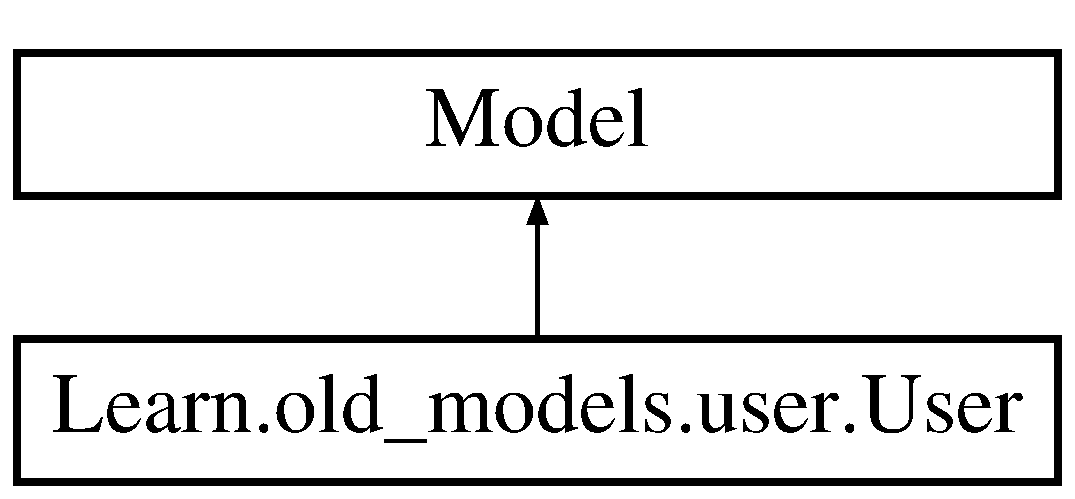
\includegraphics[height=2.000000cm]{class_learn_1_1old__models_1_1user_1_1_user}
\end{center}
\end{figure}
\subsection*{Classes}
\begin{DoxyCompactItemize}
\item 
class \hyperlink{class_learn_1_1old__models_1_1user_1_1_user_1_1_meta}{Meta}
\end{DoxyCompactItemize}
\subsection*{Public Member Functions}
\begin{DoxyCompactItemize}
\item 
\hypertarget{class_learn_1_1old__models_1_1user_1_1_user_a09b32112d5beeaec0c0229ca5bc7e126}{def {\bfseries \-\_\-\-\_\-init\-\_\-\-\_\-}}\label{class_learn_1_1old__models_1_1user_1_1_user_a09b32112d5beeaec0c0229ca5bc7e126}

\end{DoxyCompactItemize}
\subsection*{Public Attributes}
\begin{DoxyCompactItemize}
\item 
\hypertarget{class_learn_1_1old__models_1_1user_1_1_user_a894bd93cc2caf7e7a00c180f26863492}{{\bfseries uuid}}\label{class_learn_1_1old__models_1_1user_1_1_user_a894bd93cc2caf7e7a00c180f26863492}

\end{DoxyCompactItemize}
\subsection*{Static Public Attributes}
\begin{DoxyCompactItemize}
\item 
\hypertarget{class_learn_1_1old__models_1_1user_1_1_user_af60e13d947e49d668e7d9af32a9f095a}{tuple {\bfseries uuid} models.\-Char\-Field(max\-\_\-length=36, primary\-\_\-key=True)}\label{class_learn_1_1old__models_1_1user_1_1_user_af60e13d947e49d668e7d9af32a9f095a}

\item 
\hypertarget{class_learn_1_1old__models_1_1user_1_1_user_aa2c2f61f85073496e09612cd4c2abd2e}{tuple {\bfseries forename} models.\-Char\-Field(max\-\_\-length=50)}\label{class_learn_1_1old__models_1_1user_1_1_user_aa2c2f61f85073496e09612cd4c2abd2e}

\item 
\hypertarget{class_learn_1_1old__models_1_1user_1_1_user_a713f9b733aa97b1364415126b8f789a9}{tuple {\bfseries surname} models.\-Char\-Field(max\-\_\-length=50)}\label{class_learn_1_1old__models_1_1user_1_1_user_a713f9b733aa97b1364415126b8f789a9}

\item 
\hypertarget{class_learn_1_1old__models_1_1user_1_1_user_af452b5a8caef5df2d87e4c8c7f79ada0}{tuple {\bfseries username} models.\-Char\-Field(max\-\_\-length=50)}\label{class_learn_1_1old__models_1_1user_1_1_user_af452b5a8caef5df2d87e4c8c7f79ada0}

\item 
\hypertarget{class_learn_1_1old__models_1_1user_1_1_user_af6ecd12012d2cae25ada38bb93f3eb1d}{tuple {\bfseries email} models.\-Email\-Field(max\-\_\-length=254)}\label{class_learn_1_1old__models_1_1user_1_1_user_af6ecd12012d2cae25ada38bb93f3eb1d}

\item 
\hypertarget{class_learn_1_1old__models_1_1user_1_1_user_a70a55469415a167614974bdb85b0f0c9}{tuple {\bfseries phone} models.\-Char\-Field(max\-\_\-length=50)}\label{class_learn_1_1old__models_1_1user_1_1_user_a70a55469415a167614974bdb85b0f0c9}

\end{DoxyCompactItemize}


The documentation for this class was generated from the following file\-:\begin{DoxyCompactItemize}
\item 
/\-Users/\-Charlie/\-Documents/\-Aptana Studio 3 Workspace/\-C\-M2301-\/9/\-C\-M2301/\-Learn/old\-\_\-models/user.\-py\end{DoxyCompactItemize}

\hypertarget{class_learn_1_1models_1_1_user_field}{\section{Learn.\-models.\-User\-Field Class Reference}
\label{class_learn_1_1models_1_1_user_field}\index{Learn.\-models.\-User\-Field@{Learn.\-models.\-User\-Field}}
}


A \hyperlink{class_learn_1_1models_1_1_user_field}{User\-Field} is a value attached to a user.  


Inheritance diagram for Learn.\-models.\-User\-Field\-:\begin{figure}[H]
\begin{center}
\leavevmode
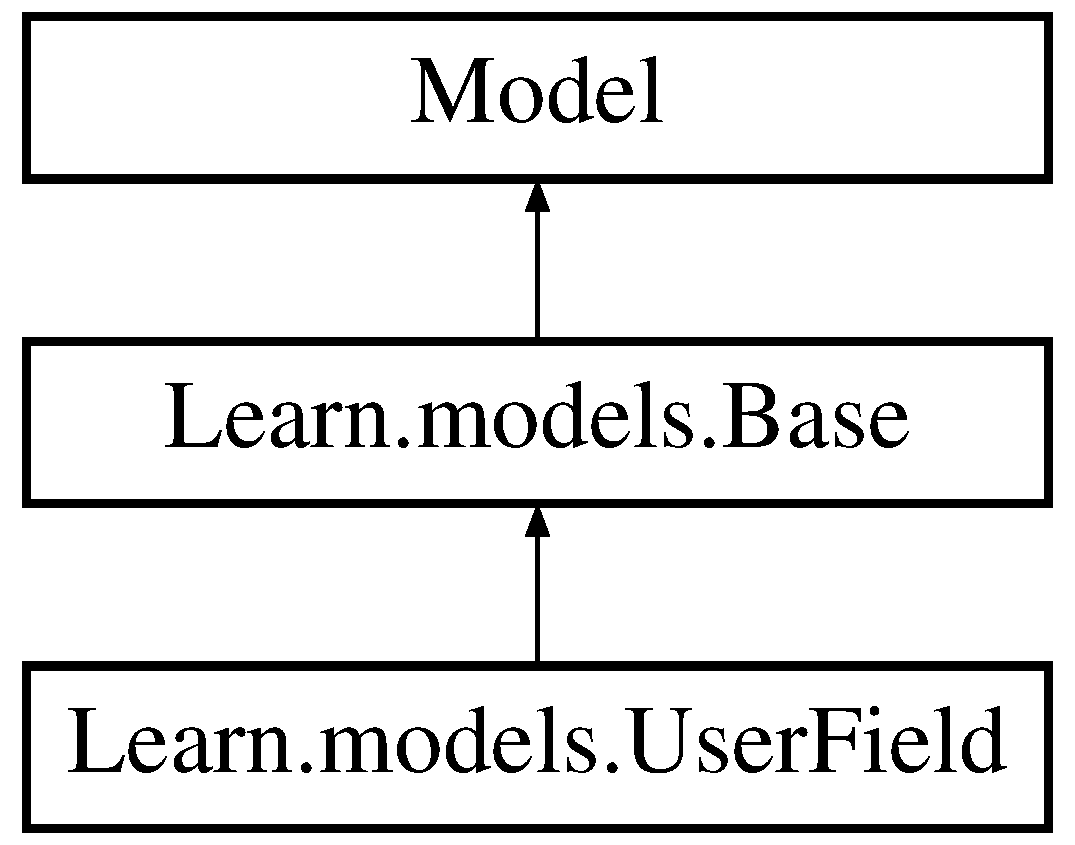
\includegraphics[height=3.000000cm]{class_learn_1_1models_1_1_user_field}
\end{center}
\end{figure}
\subsection*{Static Public Attributes}
\begin{DoxyCompactItemize}
\item 
\hypertarget{class_learn_1_1models_1_1_user_field_a0862a63a5ba3220152b87c96d36565d2}{tuple \hyperlink{class_learn_1_1models_1_1_user_field_a0862a63a5ba3220152b87c96d36565d2}{user} models.\-Foreign\-Key(\hyperlink{class_learn_1_1models_1_1_user}{User})}\label{class_learn_1_1models_1_1_user_field_a0862a63a5ba3220152b87c96d36565d2}

\begin{DoxyCompactList}\small\item\em The \hyperlink{class_learn_1_1models_1_1_user}{User} the \hyperlink{class_learn_1_1models_1_1_user_field}{User\-Field} belongs to. \end{DoxyCompactList}\item 
\hypertarget{class_learn_1_1models_1_1_user_field_a2dab1d7cf7c6fd1ab7f2811808a4f9b5}{tuple \hyperlink{class_learn_1_1models_1_1_user_field_a2dab1d7cf7c6fd1ab7f2811808a4f9b5}{key} models.\-Char\-Field(max\-\_\-length=250)}\label{class_learn_1_1models_1_1_user_field_a2dab1d7cf7c6fd1ab7f2811808a4f9b5}

\begin{DoxyCompactList}\small\item\em The field key. \end{DoxyCompactList}\item 
\hypertarget{class_learn_1_1models_1_1_user_field_a5dcb33b60bc478fcc5eaff5d526f7a71}{tuple \hyperlink{class_learn_1_1models_1_1_user_field_a5dcb33b60bc478fcc5eaff5d526f7a71}{value} models.\-Text\-Field()}\label{class_learn_1_1models_1_1_user_field_a5dcb33b60bc478fcc5eaff5d526f7a71}

\begin{DoxyCompactList}\small\item\em The field value. \end{DoxyCompactList}\end{DoxyCompactItemize}
\subsection*{Additional Inherited Members}


\subsection{Detailed Description}
A \hyperlink{class_learn_1_1models_1_1_user_field}{User\-Field} is a value attached to a user. 

Users can have multiple User\-Fields allowing for unique fields to be added to a specific \hyperlink{class_learn_1_1models_1_1_user}{User}. 

The documentation for this class was generated from the following file\-:\begin{DoxyCompactItemize}
\item 
/\-Users/\-Charlie/\-Documents/\-Aptana Studio 3 Workspace/\-C\-M2301-\/9/\-C\-M2301/\-Learn/models.\-py\end{DoxyCompactItemize}

\hypertarget{class_learn_1_1models_1_1_video}{\section{Learn.\-models.\-Video Class Reference}
\label{class_learn_1_1models_1_1_video}\index{Learn.\-models.\-Video@{Learn.\-models.\-Video}}
}


Represents a video, can contain multiple Video\-Formats.  


Inheritance diagram for Learn.\-models.\-Video\-:\begin{figure}[H]
\begin{center}
\leavevmode
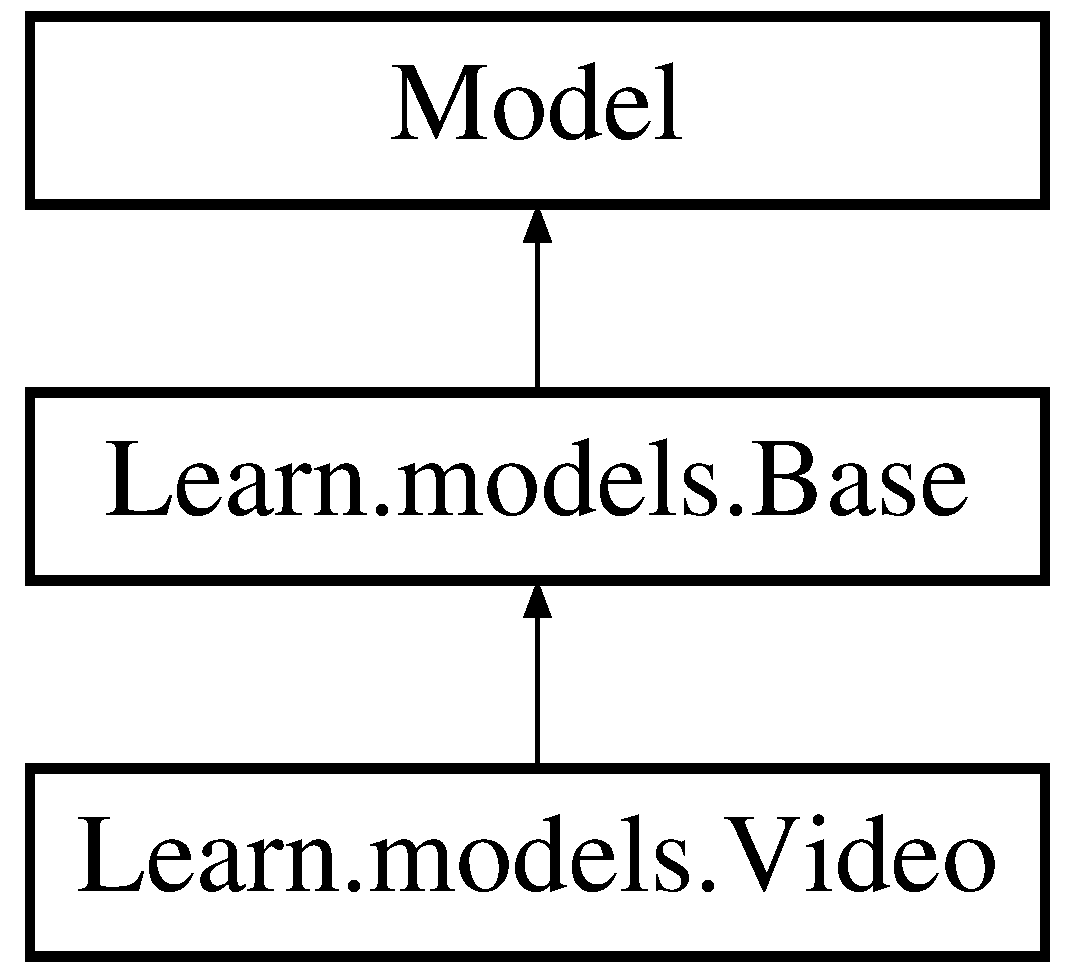
\includegraphics[height=3.000000cm]{class_learn_1_1models_1_1_video}
\end{center}
\end{figure}
\subsection*{Public Member Functions}
\begin{DoxyCompactItemize}
\item 
\hypertarget{class_learn_1_1models_1_1_video_a45139e19d67924b2afee255d5e6d35ff}{def \hyperlink{class_learn_1_1models_1_1_video_a45139e19d67924b2afee255d5e6d35ff}{get\-\_\-file\-\_\-paths}}\label{class_learn_1_1models_1_1_video_a45139e19d67924b2afee255d5e6d35ff}

\begin{DoxyCompactList}\small\item\em Returns a dictionary of filepaths for every availiable format. \end{DoxyCompactList}\item 
\hypertarget{class_learn_1_1models_1_1_video_a23fa5974b44b04711871a2f3a788da7d}{def \hyperlink{class_learn_1_1models_1_1_video_a23fa5974b44b04711871a2f3a788da7d}{get\-\_\-file\-\_\-path}}\label{class_learn_1_1models_1_1_video_a23fa5974b44b04711871a2f3a788da7d}

\begin{DoxyCompactList}\small\item\em Returns the video file path for the specified format. \end{DoxyCompactList}\end{DoxyCompactItemize}
\subsection*{Static Public Attributes}
\begin{DoxyCompactItemize}
\item 
\hypertarget{class_learn_1_1models_1_1_video_a7c34eae5bb8e4c32a2b45ad5418b78ad}{tuple {\bfseries title} models.\-Char\-Field(max\-\_\-length=50)}\label{class_learn_1_1models_1_1_video_a7c34eae5bb8e4c32a2b45ad5418b78ad}

\item 
\hypertarget{class_learn_1_1models_1_1_video_a77bf282342a37c639a0c017c98a49c8a}{tuple {\bfseries description} models.\-Text\-Field()}\label{class_learn_1_1models_1_1_video_a77bf282342a37c639a0c017c98a49c8a}

\end{DoxyCompactItemize}


\subsection{Detailed Description}
Represents a video, can contain multiple Video\-Formats. 

Contains video title, keywords and description. 

The documentation for this class was generated from the following file\-:\begin{DoxyCompactItemize}
\item 
/\-Users/\-Charlie/\-Documents/\-Aptana Studio 3 Workspace/\-C\-M2301-\/9/\-C\-M2301/\-Learn/models.\-py\end{DoxyCompactItemize}

\hypertarget{class_learn_1_1models_1_1_video_format}{\section{Learn.\-models.\-Video\-Format Class Reference}
\label{class_learn_1_1models_1_1_video_format}\index{Learn.\-models.\-Video\-Format@{Learn.\-models.\-Video\-Format}}
}


Repersents a specific format converted video file belongs to a video object.  


Inheritance diagram for Learn.\-models.\-Video\-Format\-:\begin{figure}[H]
\begin{center}
\leavevmode
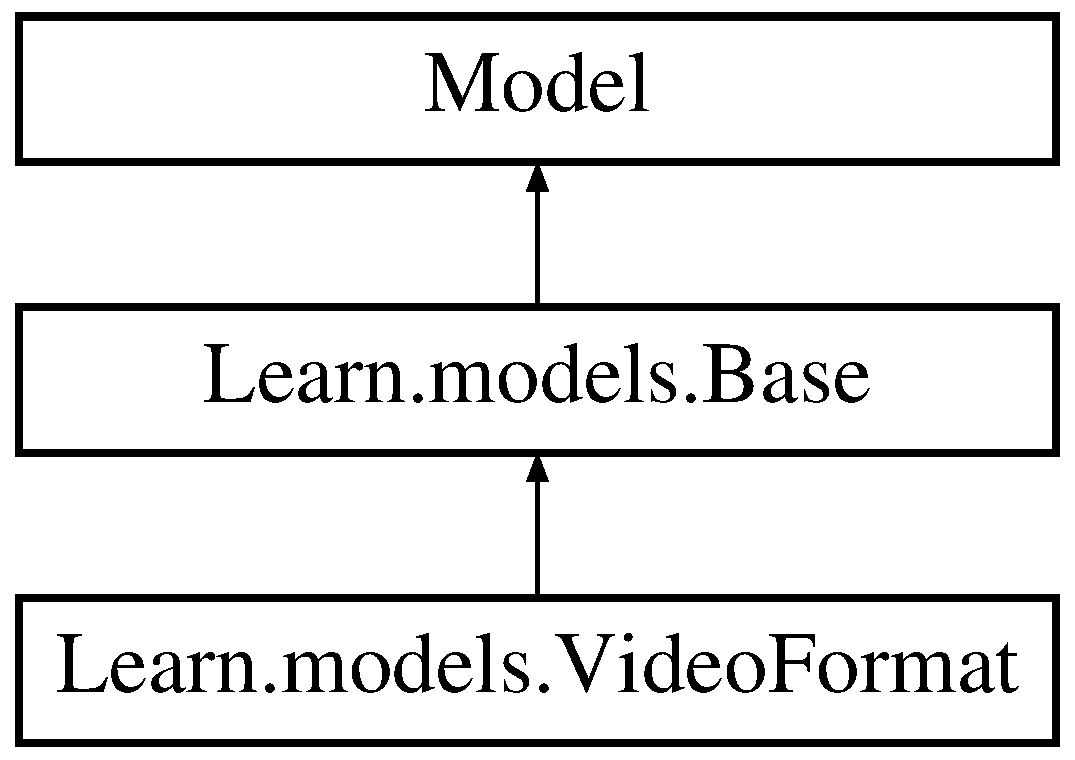
\includegraphics[height=3.000000cm]{class_learn_1_1models_1_1_video_format}
\end{center}
\end{figure}
\subsection*{Public Member Functions}
\begin{DoxyCompactItemize}
\item 
def \hyperlink{class_learn_1_1models_1_1_video_format_a47585f10ca027ae67635924ec4fd616a}{probe}
\begin{DoxyCompactList}\small\item\em Return ffprobe class from video. \end{DoxyCompactList}\end{DoxyCompactItemize}
\subsection*{Static Public Attributes}
\begin{DoxyCompactItemize}
\item 
\hypertarget{class_learn_1_1models_1_1_video_format_a2ad0de1d0c37e6262ffb11445a6812a5}{tuple {\bfseries format} models.\-Char\-Field(max\-\_\-length=20)}\label{class_learn_1_1models_1_1_video_format_a2ad0de1d0c37e6262ffb11445a6812a5}

\item 
\hypertarget{class_learn_1_1models_1_1_video_format_a7540588a59edfb8d6bd191bd524801f4}{tuple {\bfseries encoding} models.\-Char\-Field(max\-\_\-length=50)}\label{class_learn_1_1models_1_1_video_format_a7540588a59edfb8d6bd191bd524801f4}

\item 
\hypertarget{class_learn_1_1models_1_1_video_format_a8888bbfb1040d6defa7bdcfd02c21a45}{tuple {\bfseries bitrate} models.\-Char\-Field(max\-\_\-length=10)}\label{class_learn_1_1models_1_1_video_format_a8888bbfb1040d6defa7bdcfd02c21a45}

\item 
\hypertarget{class_learn_1_1models_1_1_video_format_af6905bcf941ab6e7d9475a08ebbb9c80}{tuple {\bfseries file} models.\-File\-Field(upload\-\_\-to='/')}\label{class_learn_1_1models_1_1_video_format_af6905bcf941ab6e7d9475a08ebbb9c80}

\end{DoxyCompactItemize}


\subsection{Detailed Description}
Repersents a specific format converted video file belongs to a video object. 

\subsection{Member Function Documentation}
\hypertarget{class_learn_1_1models_1_1_video_format_a47585f10ca027ae67635924ec4fd616a}{\index{Learn\-::models\-::\-Video\-Format@{Learn\-::models\-::\-Video\-Format}!probe@{probe}}
\index{probe@{probe}!Learn::models::VideoFormat@{Learn\-::models\-::\-Video\-Format}}
\subsubsection[{probe}]{\setlength{\rightskip}{0pt plus 5cm}def Learn.\-models.\-Video\-Format.\-probe (
\begin{DoxyParamCaption}
\item[{}]{self}
\end{DoxyParamCaption}
)}}\label{class_learn_1_1models_1_1_video_format_a47585f10ca027ae67635924ec4fd616a}


Return ffprobe class from video. 



The documentation for this class was generated from the following file\-:\begin{DoxyCompactItemize}
\item 
/\-Users/\-Charlie/\-Documents/\-Aptana Studio 3 Workspace/\-C\-M2301-\/9/\-C\-M2301/\-Learn/models.\-py\end{DoxyCompactItemize}

\addcontentsline{toc}{part}{Index}
\printindex
\end{document}
